\documentclass[journal,12pt,onecolumn]{IEEEtran}
\usepackage{cite}
 \usepackage{caption}
\usepackage{graphicx}
\usepackage{amsmath,amssymb,amsfonts,amsthm}
\usepackage{algorithmic}
\usepackage{graphicx}
\usepackage{textcomp}
\usepackage{xcolor}
\usepackage{txfonts}
\usepackage{listings}
\usepackage{enumitem}
\usepackage{mathtools}
\usepackage{gensymb}
\usepackage{comment}
\usepackage[breaklinks=true]{hyperref}
\usepackage{tkz-euclide} 
\usepackage{listings}
\usepackage{gvv}                                        
%\def\inputGnumericTable{}                                 
\usepackage[latin1]{inputenc} 
\usetikzlibrary{arrows.meta, positioning}
\usepackage{xparse}
\usepackage{color}                                            
\usepackage{array}                                            
\usepackage{longtable}                                       
\usepackage{calc}                                             
\usepackage{multirow}
\usepackage{multicol}
\usepackage{hhline}                                           
\usepackage{ifthen}                                           
\usepackage{lscape}
\usepackage{tabularx}
\usepackage{array}
\usepackage{float}
\newtheorem{theorem}{Theorem}[section]
\newtheorem{problem}{Problem}
\newtheorem{proposition}{Proposition}[section]
\newtheorem{lemma}{Lemma}[section]
\newtheorem{corollary}[theorem]{Corollary}
\newtheorem{example}{Example}[section]
\newtheorem{definition}[problem]{Definition}
\newcommand{\BEQA}{\begin{eqnarray}}
\newcommand{\EEQA}{\end{eqnarray}}
\usepackage{float}
\graphicspath{{./figs/}}
%\newcommand{\define}{\stackrel{\triangle}{=}}
\theoremstyle{remark}
\usepackage{circuitikz}
\captionsetup{justification=centering}
\usepackage{tikz}


\title{EC: ELECTRONICS AND COMMUNICATION ENGINEERING - 2025}
\author{EE25BTECH11037 - Divyansh}

\begin{document}
\maketitle
\begin{enumerate}

\item Here are two analogous groups, Group-I and Group-II, that list words in their decreasing order of intensity. Identify the missing word in Group-II. 

Group-I: Abuse $\rightarrow$ Insult $\rightarrow$ Ridicule 

Group-II: \underline{\hspace{2cm}} $\rightarrow$ Praise $\rightarrow$ Appreciate

\hfill{\brak{\text{GATE EC 2025}}}

\begin{enumerate}
\begin{multicols}{4}
\item Extol
\item Prize
\item Appropriate
\item Espouse
\end{multicols}
\end{enumerate}

\item Had I learnt acting as a child, I \underline{\hspace{2cm}} a famous film star. 

Select the most appropriate option to complete the above sentence.

\hfill{\brak{\text{GATE EC 2025}}}
\begin{enumerate}
\begin{multicols}{4}
\item will be
\item can be
\item am going to be
\item could have been
\end{multicols}
\end{enumerate}

\item The $12$ musical notes are given as C, $C^{\#}$ D, $D^{\#}$, E, F, $F^{\#}$, $G,$ $G^{\#}$, A, $A^{\#},$ and B. Frequency of each note is $\sqrt[12]{2}$ times the frequency of the previous note. If the frequency of the note C is $130.8$ Hz, then the ratio of frequencies of notes $F^{\#}$ and C is:

\hfill{\brak{\text{GATE EC 2025}}}

\begin{enumerate}
\begin{multicols}{4}
\item $\sqrt[6]{2}$
\item $\sqrt{2}$
\item $\sqrt[4]{2}$
\item $2$
\end{multicols}
\end{enumerate}

\item The following $\figref{fig:q4}$ show three curves generated using an iterative algorithm. The total length of the curve generated after 'Iteration $n'$ is:
\begin{figure}[H]
\centering
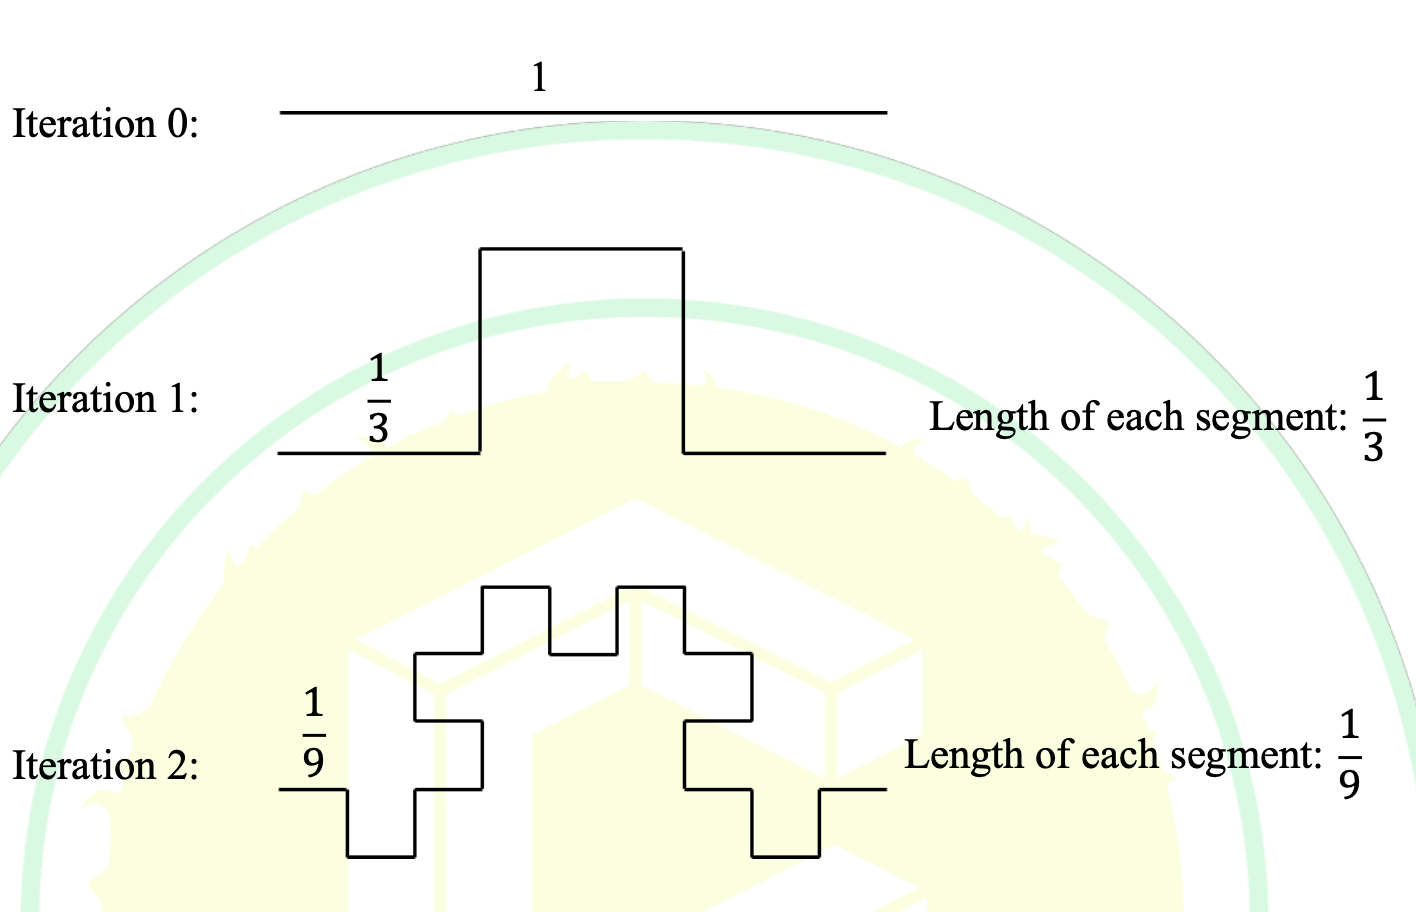
\includegraphics[width=0.6\columnwidth]{q4}
\caption{For q-4}
\label{fig:q4}
\end{figure}

\hfill{\brak{\text{GATE EC 2025}}}

\begin{enumerate}
\begin{multicols}{4}
\item $\brak{\dfrac{5}{3}}^{\frac{n}{2}}$
\item $\brak{\dfrac{5}{3}}^{n}$
\item $\brak{\dfrac{5}{3}}$
\item $\brak{\dfrac{5}{3}}^{n\brak{2n-1}}$
\end{multicols}
\end{enumerate}

\item Which one of the following plots represents $f\brak{x}=-\dfrac{\abs{x}}{x},$ where $x$ is a non-zero real number?

\hfill{\brak{\text{GATE EC 2025}}}

\begin{multicols}{4}
\begin{enumerate}
    \item 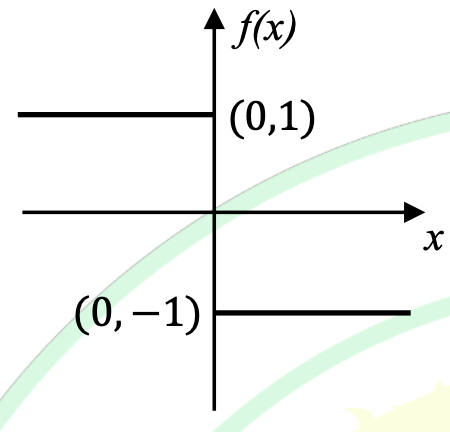
\includegraphics[width=0.4\columnwidth]{q5a.png}
    \item 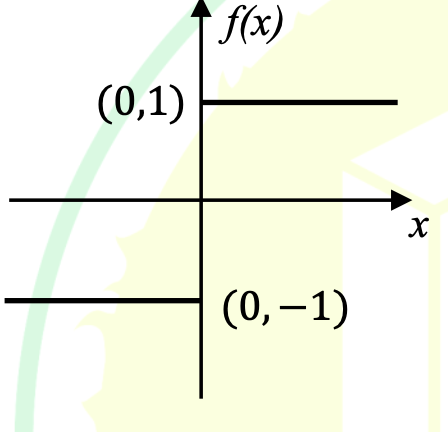
\includegraphics[width=0.4\columnwidth]{q5b.png}
    \item 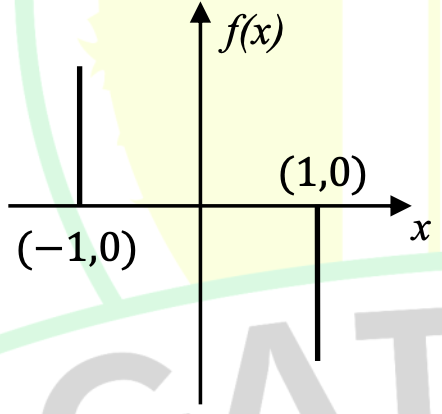
\includegraphics[width=0.4\columnwidth]{q5c.png}
    \item 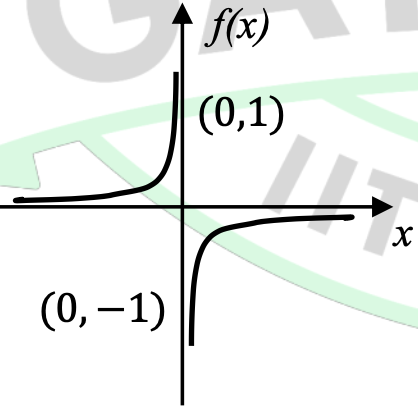
\includegraphics[width=0.4\columnwidth]{q5d.png}
\end{enumerate}
\end{multicols}


\item Identify the option that has the most appropriate sequence such that a coherent paragraph is formed: \\
\begin{enumerate}[start=16,label=\Alph*.]
    \item Over time, such adaptations lead to significant evolutionary changes with the potential to shape the development of new species.
    \item In natural world, organisms constantly adapt to their environments in response to challenges and opportunities.
    \item This process of adaptation is driven by the principle of natural selection, where favorable traits increase an organism's chances of survival and reproduction.
    \item As environments change, organisms that can adapt their behavior, structure and physiology to such changes are more likely to survive.
\end{enumerate}

\hfill{\brak{\text{GATE EC 2025}}}

\begin{enumerate}
\begin{multicols}{4}
\item $P\rightarrow Q\rightarrow R\rightarrow S$
\item $Q\rightarrow S\rightarrow R\rightarrow P$
\item $R\rightarrow S\rightarrow Q\rightarrow P$
\item $S\rightarrow P\rightarrow R\rightarrow Q$
\end{multicols}
\end{enumerate}

\item A stick of length one meter is broken at two locations at distances of $b_{1}$ and $b_{2}$ from the origin $\brak{0}$, as shown in the $\figref{fig:q7}$. Note that $0<b_{1}<b_{2}<1$. Which one of the following is NOT a necessary condition for forming a triangle using the three pieces?
\begin{figure}[H]
\centering
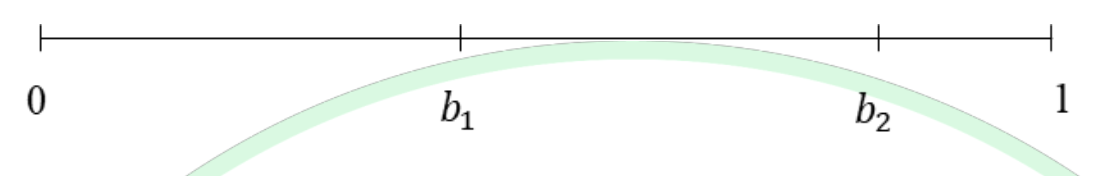
\includegraphics[width=0.7\columnwidth]{q7}
\caption{For q-7}
\label{fig:q7}
\end{figure}

\hfill{\brak{\text{GATE EC 2025}}}

\begin{enumerate}
\begin{multicols}{4}
\item $b_{1}<0.5$
\item $b_{2}>0.5$
\item $b_{2}<b_{1}+0.5$
\item $b_{1}+b_{2}<1$
\end{multicols}
\end{enumerate}

\item Eight students $\brak{P, Q, R, S, T, U, V, \text{ and } W}$ are playing musical chairs. The $\figref{fig:q8}$ indicates their order of position at the start of the game. They play the game by moving forward in a circle in the clockwise direction. After the $1^{st}$ round, $4^{th}$ student behind P leaves the game. After $2^{nd}$ round, $5^{th}$ student behind Q leaves the game. After $3^{rd}$ round, $3^{rd}$ student behind V leaves the game. After $4^{th}$ round, $4^{th}$ student behind U leaves the game. Who all are left in the game after the $4^{th}$ round?
\begin{figure}[H]
\centering
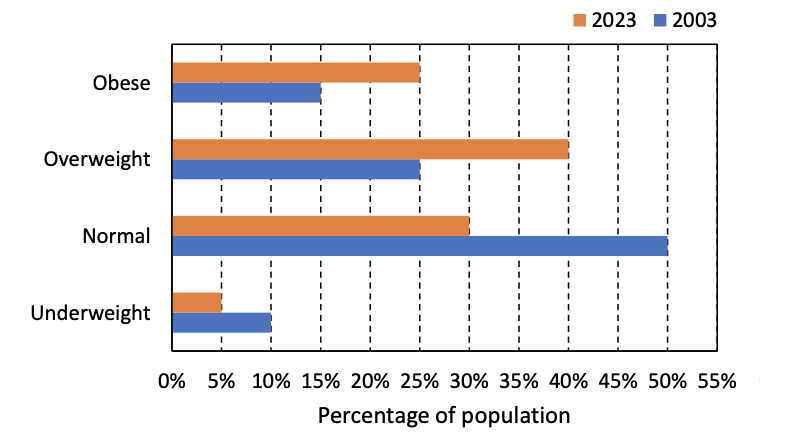
\includegraphics[width=0.4\columnwidth]{q8}
\caption{For q-8}
\label{fig:q8}
\end{figure}

\hfill{\brak{\text{GATE EC 2025}}}

\begin{enumerate}
\begin{multicols}{4}
\item P; T; Q; S
\item V; P; T; Q
\item W; R; Q; U
\item Q; T; V; W
\end{multicols}
\end{enumerate}

\item The table lists the top 5 nations according to the number of gold medals won in a tournament; also included are the number of silver and the bronze medals won by them. Based only on the data provided in the table, which one of the following statements is INCORRECT?
\begin{table}[h]
\centering
\begin{tabular}{|l|c|c|c|}
\hline
\textbf{Nation} & \textbf{Gold} & \textbf{Silver} & \textbf{Bronze} \\ \hline
USA & 40 & 44 & 41 \\
Canada & 39 & 24 & 27 \\
Japan & 12 & 20 & 13 \\
Australia & 19 & 17 & 16 \\
France & 16 & 22 & 26 \\ \hline
\end{tabular}
\caption*{}
\label{tab:q9}
\end{table}

\hfill{\brak{\text{GATE EC 2025}}}

\begin{enumerate}
\item France will occupy the third place if the list were made on the basis of the total number of medals won.
\item The order of the top two nations will not change even if the list is made on the basis of the total number of medals won.
\item USA and Canada together have less than 50\% of the medals awarded to the nations in the above table.
\item Canada has won twice as many total medals as Japan.
\end{enumerate}

\item An organization allows its employees to work independently on consultancy projects but charges an overhead on the consulting fee. The overhead is $20\%$ of the consulting fee, if the fee is up to 4. For higher fees, the overhead is $1,00,000$ plus $10\%$ of the amount by which the fee exceeds $5,00,000$. The government charges a Goods and Services Tax of $18\%$ on the total amount $\brak{\text{the consulting fee plus the overhead}}$. An employee of the organization charges this entire amount, i.e., the consulting fee, overhead, and tax, to the client. If the client cannot pay more than $10,00,000$, what is the maximum consulting fee that the employee can charge?

\hfill{\brak{\text{GATE EC 2025}}}

\begin{enumerate}
\begin{multicols}{4}
\item 7,01,438
\item 7,24,961
\item 7,51,232
\item 7,75,784
\end{multicols}
\end{enumerate}

\item Consider the matrix A below:
\[ A=\myvec{2&3&4&5\\ 0&6&7&8\\ 0&0&\alpha&\beta\\ 0&0&0&\gamma} \]
For which of the following combinations of $\alpha$, $\beta$, and $\gamma$, is the rank of A at least three? 
\begin{enumerate}[label=(\roman*)]
    \item $\alpha=0$ and $\beta=\gamma\ne0$.
    \item $\alpha=\beta=\gamma=0$
    \item $\beta=\gamma=0$ and $\alpha\ne0$.
    \item $\alpha=\beta=\gamma\ne0$
\end{enumerate}


\hfill{\brak{\text{GATE EC 2025}}}

\begin{enumerate}
\begin{multicols}{4}
\item Only (i), (iii), and (iv)
\item Only (iv)
\item Only (ii)
\item Only (i) and (iii)
\end{multicols}
\end{enumerate}

\item Consider the following series: 
\begin{align*}
    (i) \sum_{n=1}^{\infty} \frac{1}{\sqrt{n}} \quad (ii) \sum_{n=1}^{\infty} \frac{1}{n\brak{n+1}} \quad (iii) \sum_{n=1}^{\infty} \frac{1}{n!}
\end{align*}
Choose the correct option.

\hfill{\brak{\text{GATE EC 2025}}}

\begin{enumerate}
\begin{multicols}{2}
\item Only (ii) converges
\item Only (ii) and (iii) converge
\item Only (iii) converges
\item All three converge
\end{multicols}
\end{enumerate}

\item A pot contains two red balls and two blue balls. Two balls are drawn from this pot randomly without replacement. What is the probability that the two balls drawn have different colours?

\hfill{\brak{\text{GATE EC 2025}}}

\begin{enumerate}
\begin{multicols}{4}
\item $2/3$
\item $1/3$
\item $1/2$
\item $1$
\end{multicols}
\end{enumerate}

\item Consider a frequency-modulated $\brak{FM}$ signal $f\brak{t} = A_c \cos\brak{2\pi f_c t + 3 \sin\brak{2\pi f_1 t} + 4 \sin\brak{6\pi f_1 t}}$, where $A_c$ and $f_c$ are, respectively, the amplitude and frequency $\brak{\text{in Hz}}$ of the carrier waveform. The frequency $f_1$ is in Hz, and assume that $f_c > 100f_1$. The peak frequency deviation of the FM signal in Hz is \underline{\hspace{2cm}}.

\hfill{\brak{\text{GATE EC 2025}}}

\begin{enumerate}
\begin{multicols}{4}
\item $15f_1$
\item $12f_1$
\item $4f_1$
\item $2f_1$
\end{multicols}
\end{enumerate}

\item Consider an additive white Gaussian noise $\brak{AWGN}$ channel with bandwidth $W$ and noise power spectral density $\frac{N_0}{2}$. Let $P_{av}$ denote the average transmit power constraint. Which one of the following plots illustrates the dependence of the channel capacity $C$ on the bandwidth $W$ $\brak{\text{keeping } P_{av} \text{ and } N_0 \text{ fixed}}$?

\hfill{\brak{\text{GATE EC 2025}}}

\begin{multicols}{2}
\begin{enumerate}
    \item 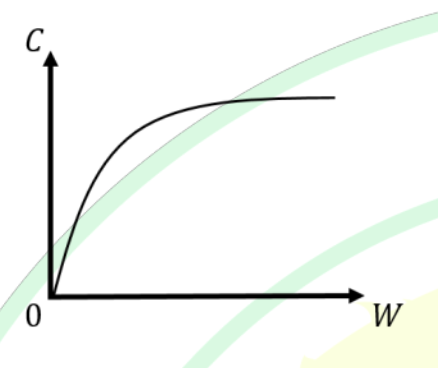
\includegraphics[width=0.3\columnwidth]{q15a.png}
    \item 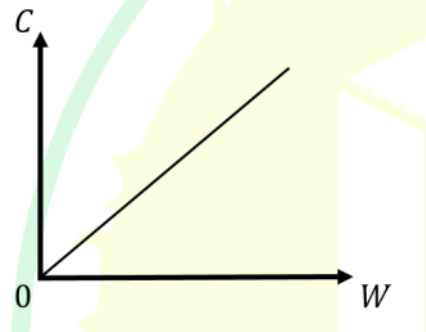
\includegraphics[width=0.3\columnwidth]{q15b.png}
    \item 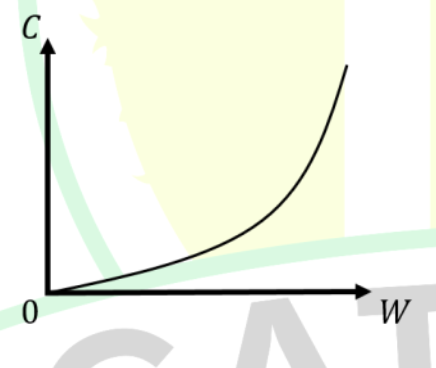
\includegraphics[width=0.3\columnwidth]{q15c.png}
    \item 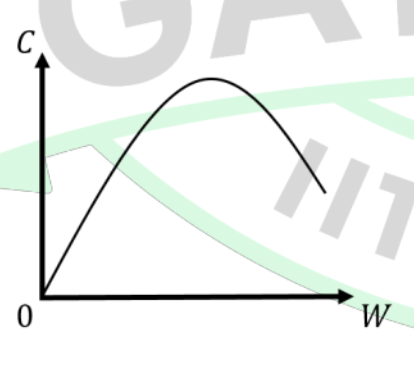
\includegraphics[width=0.3\columnwidth]{q15d.png}
\end{enumerate}
\end{multicols}


\item The Nyquist plot of a system is given in the $\figref{fig:q16}$ below. Let $\omega_P, \omega_Q, \omega_R,$ and $\omega_S$ be the positive frequencies at the points $P, Q, R,$ and $S$, respectively. Which one of the following statements is TRUE?
\begin{figure}[H]
\centering
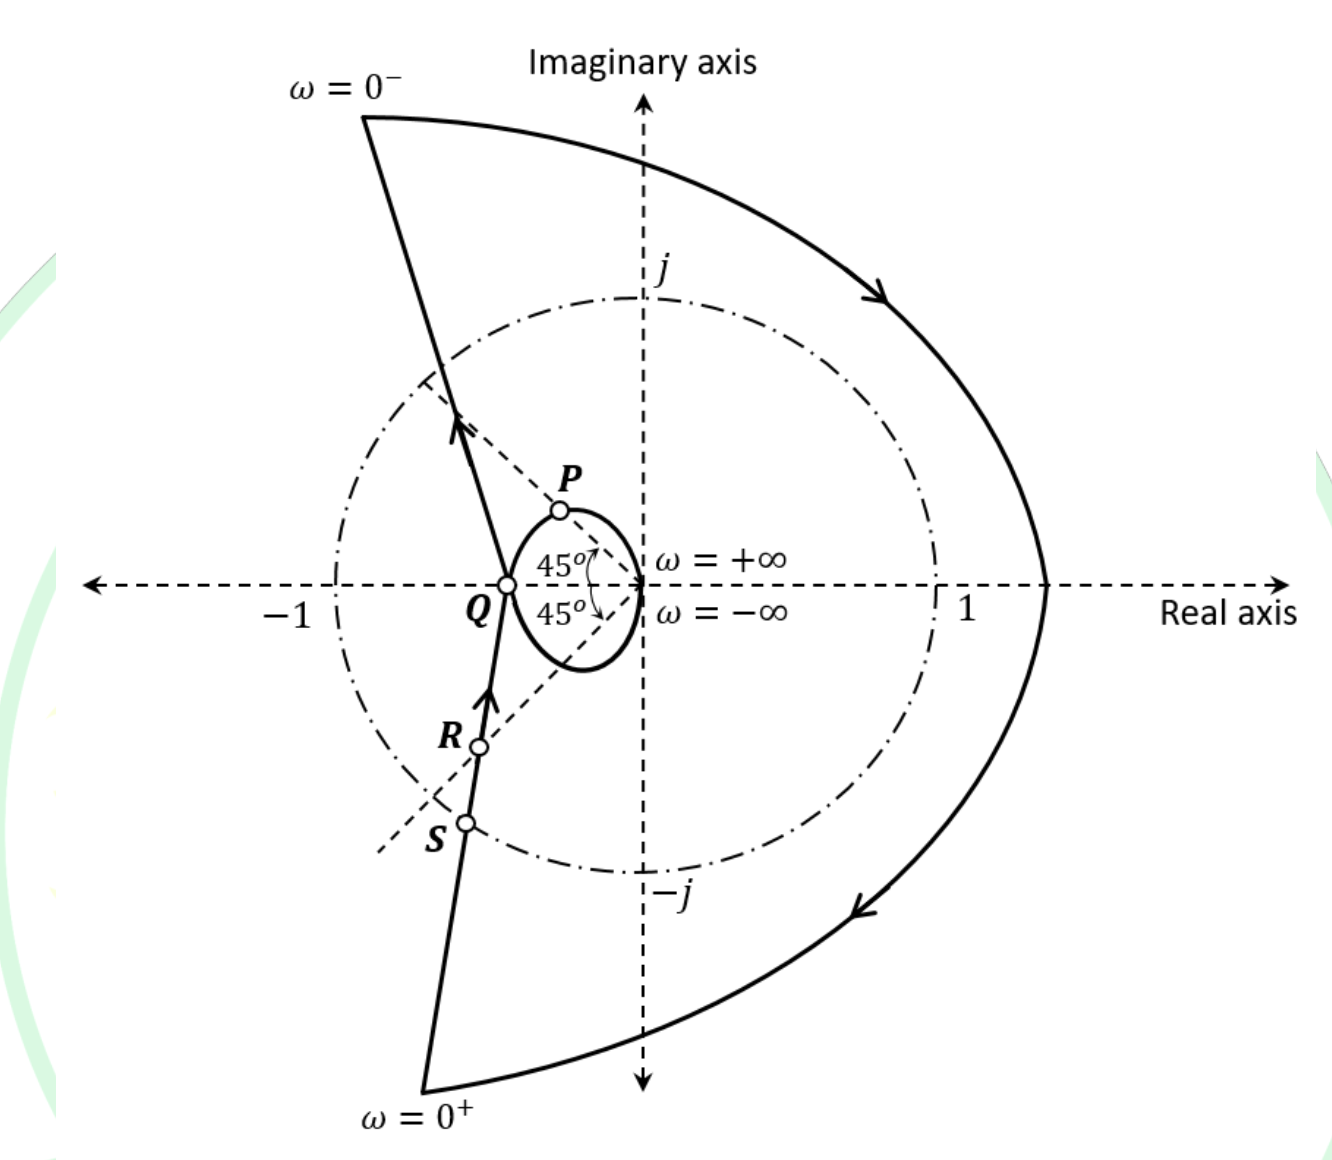
\includegraphics[width=0.5\columnwidth]{q16}
\caption{For q-16}
\label{fig:q16}
\end{figure}

\hfill{\brak{\text{GATE EC 2025}}}

\begin{enumerate}
\item $\omega_S$ is the gain crossover frequency and $\omega_P$ is the phase crossover frequency
\item $\omega_Q$ is the gain crossover frequency and $\omega_R$ is the phase crossover frequency
\item $\omega_Q$ is the gain crossover frequency and $\omega_S$ is the phase crossover frequency
\item $\omega_S$ is the gain crossover frequency and $\omega_Q$ is the phase crossover frequency
\end{enumerate}

\item Consider the discrete-time system below in $\figref{fig:q17}$ with input $x\sbrak{n}$ and output $y\sbrak{n}$. In the figure, $h_1\sbrak{n}$ and $h_2\sbrak{n}$ denote the impulse responses of LTI Subsystems 1 and 2, respectively. Also, $\delta\sbrak{n}$ is the unit impulse, and $b > 0$. Assuming $h_2\sbrak{n} \neq \delta\sbrak{n}$, the overall system $\brak{\text{denoted by the dashed box}}$ is \underline{\hspace{2cm}}.
\begin{figure}[H]
\centering
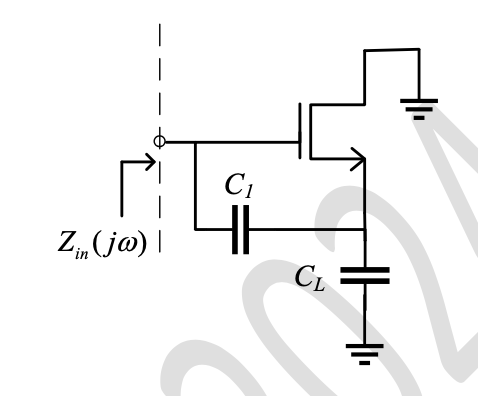
\includegraphics[width=0.5\columnwidth]{q17}
\caption{For q-17}
\label{fig:q17}
\end{figure}

\hfill{\brak{\text{GATE EC 2025}}}

\begin{enumerate}
\begin{multicols}{2}
\item linear and time invariant
\item linear and time variant
\item nonlinear and time invariant
\item nonlinear and time variant
\end{multicols}
\end{enumerate}

\item Consider a continuous-time, real-valued signal $f\brak{t}$ whose Fourier transform $F\brak{\omega} = \int_{-\infty}^{\infty} f\brak{t} \exp\brak{-j \omega t} dt$ exists. Which one of the following statements is always TRUE?

\hfill{\brak{\text{GATE EC 2025}}}
\begin{multicols}{2}
\begin{enumerate}
\item $\abs{F\brak{\omega}} \le \int_{-\infty}^{\infty} \abs{f\brak{t}} dt$
\item $\abs{F\brak{\omega}} > \int_{-\infty}^{\infty} \abs{f\brak{t}} dt$
\item $\abs{F\brak{\omega}} \le \int_{-\infty}^{\infty} f\brak{t} dt$
\item $\abs{F\brak{\omega}} \ge \int_{-\infty}^{\infty} f\brak{t} dt$
\end{enumerate} 
\end{multicols}


\item Consider a part of an electrical network as shown below in $\figref{fig:q19}$. Some node voltages, and the current flowing through the $3 \ohm$ resistor are as indicated. The voltage $\brak{\text{in Volts}}$ at node $X$ is \underline{\hspace{2cm}}.
\begin{figure}[H]
\centering
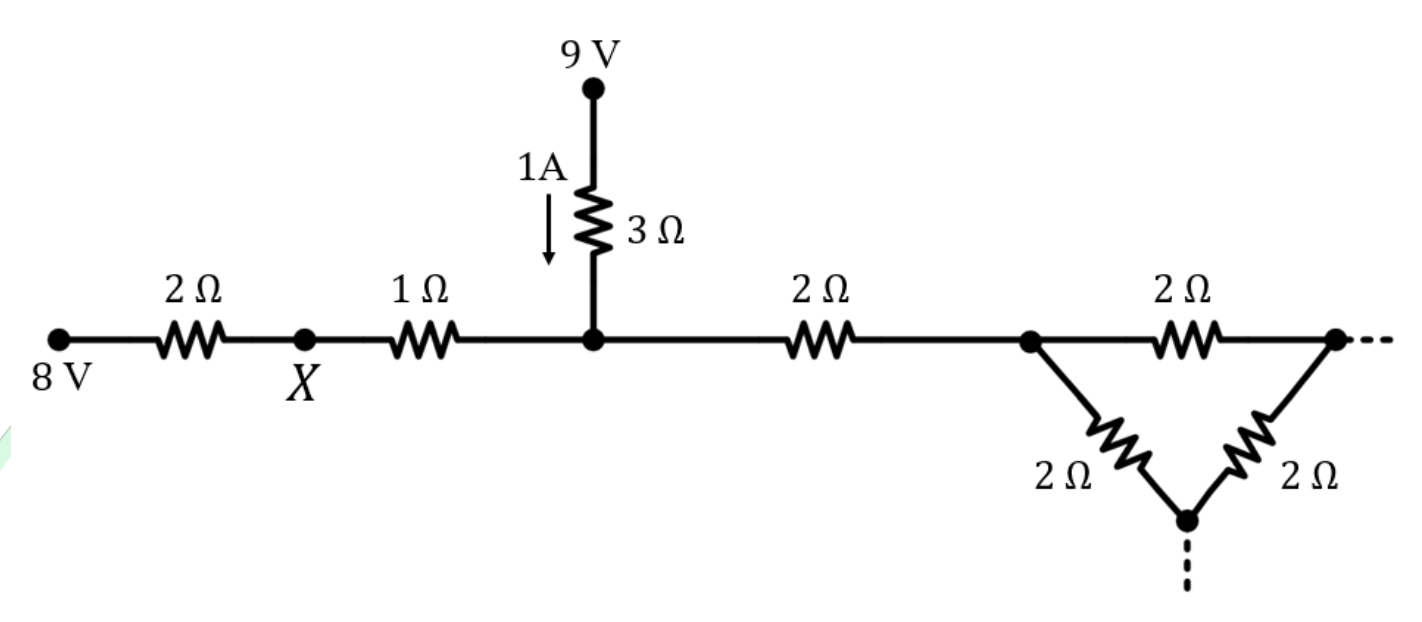
\includegraphics[width=0.6\columnwidth]{q19}
\caption{For q-19}
\label{fig:q19}
\end{figure}

\hfill{\brak{\text{GATE EC 2025}}}

\begin{enumerate}
\begin{multicols}{4}
\item $20/3$
\item $32/3$
\item $22/3$
\item $2/3$
\end{multicols}
\end{enumerate}

\item Let $i_C, i_L,$ and $i_R$ be the currents flowing through the capacitor, inductor, and resistor, respectively, in the circuit given in $\figref{fig:q20}$. The AC admittances are given in Siemens $\brak{S}$. Which one of the following is TRUE?
\begin{figure}[H]
\centering
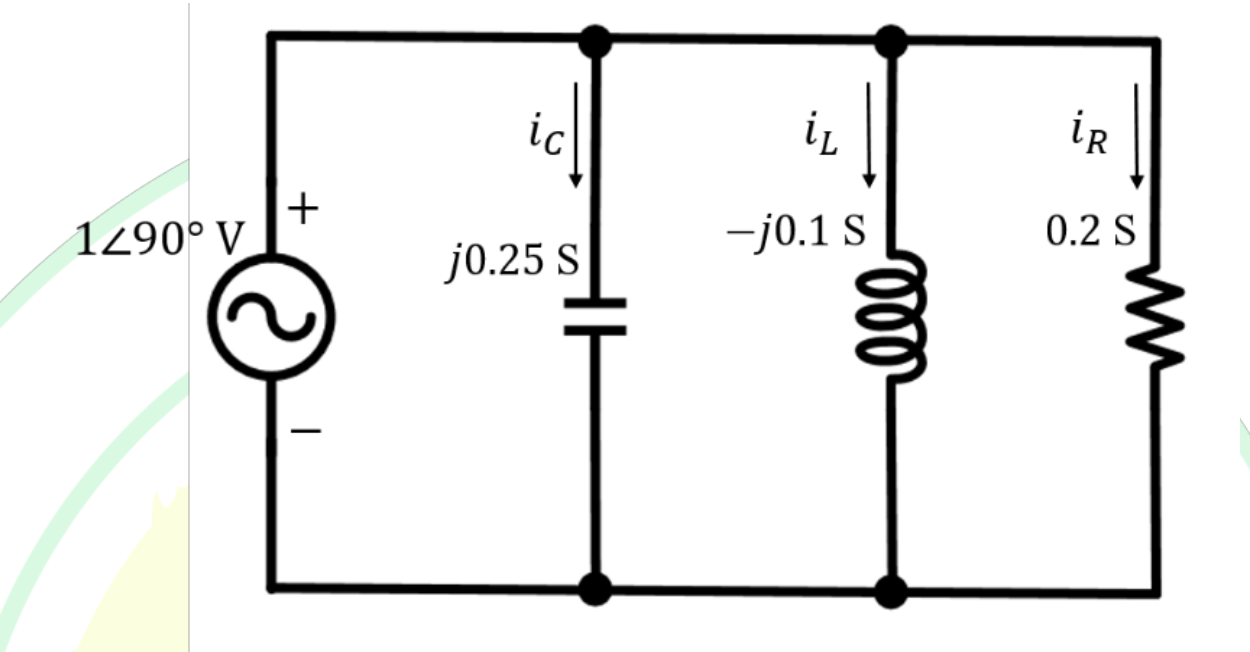
\includegraphics[width=0.5\columnwidth]{q20}
\caption{For q-20}
\label{fig:q20}
\end{figure}

\hfill{\brak{\text{GATE EC 2025}}}

\begin{enumerate}
\item $i_C = 0.25\angle180\degree$ A, $i_L = 0.1\angle0\degree$ A, $i_R = 0.2\angle90\degree$ A
\item $i_C = 4\angle180\degree$ A, $i_L = 10\angle0\degree$ A, $i_R = 5\angle90\degree$ A
\item $i_C = 0.25\angle270\degree$ A, $i_L = 0.1\angle90\degree$ A, $i_R = 0.2\angle90\degree$ A
\item $i_C = 4\angle90\degree$ A, $i_L = 10\angle270\degree$ A, $i_R = 5\angle0\degree$ A
\end{enumerate}

\item A simplified small-signal equivalent circuit of a BJT-based amplifier is given in $\figref{fig:q21}$. The small-signal voltage gain $v_o/v_s$ $\brak{\text{in V/V}}$ is \underline{\hspace{2cm}}.
\begin{figure}[H]
\centering
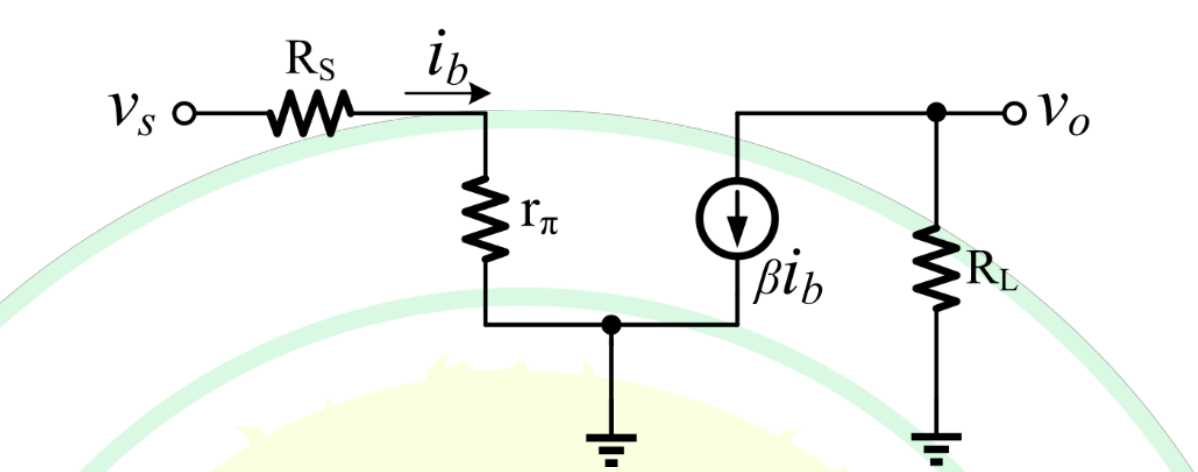
\includegraphics[width=0.5\columnwidth]{q21}
\caption{For q-21}
\label{fig:q21}
\end{figure}

\hfill{\brak{\text{GATE EC 2025}}}

\begin{enumerate}
\begin{multicols}{4}
\item $-\dfrac{\beta R_L}{R_S + r_\pi}$
\item $+\dfrac{\beta R_L}{R_S}$
\item $-\dfrac{\beta R_L}{R_S}$
\item $+\dfrac{\beta R_L}{R_S + r_\pi}$
\end{multicols}
\end{enumerate}

\item The ideal BJT in the circuit given in $\figref{fig:q22}$ is biased in the active region with a $\beta$ of $100$. If $I_B$ is $10$ \textmu A, then $V_{CE}$ $\brak{\text{in Volts, rounded off to two decimal places}}$ is \underline{\hspace{2cm}}.
\begin{figure}[H]
\centering
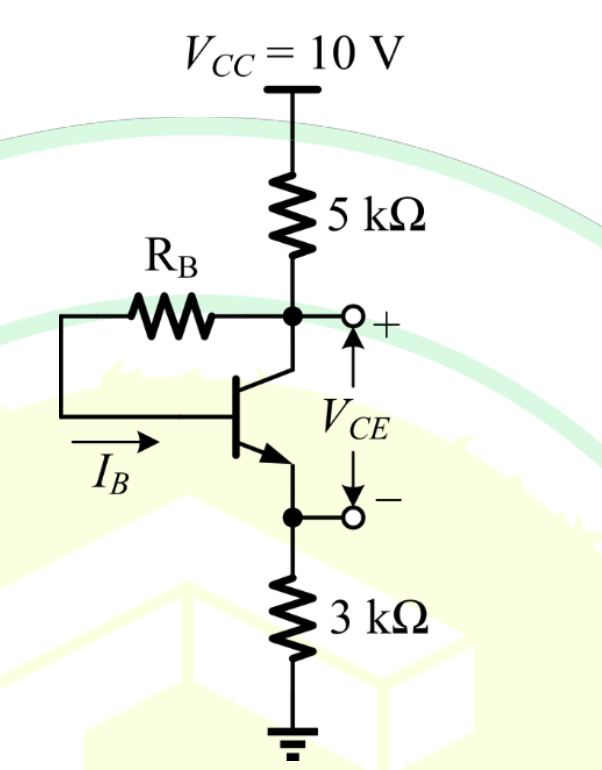
\includegraphics[width=0.3\columnwidth]{q22}
\caption{For q-22}
\label{fig:q22}
\end{figure}

\hfill{\brak{\text{GATE EC 2025}}}

\begin{enumerate}
\begin{multicols}{4}
\item $4.95$
\item $3.03$
\item $1.92$
\item $3.73$
\end{multicols}
\end{enumerate}

\item A 3-input majority logic gate has inputs $X, Y,$ and $Z$. 
    The output $F$ of the gate is logic `1` if two or more of the inputs are logic `1`. 
    The output $F$ is logic `0` if two or more of the inputs are logic `0`. 
    Which one of the following options is a Boolean expression of the output $F$?

\hfill{\brak{\text{GATE EC 2025}}}

\begin{enumerate}
\begin{multicols}{4}
\item $XY + YZ + ZX$
\item $X \oplus Y \oplus Z$
\item $X + Y + Z$
\item $XYZ$
\end{multicols}
\end{enumerate}

\item A full adder and an XOR gate are used to design a digital circuit with inputs X, Y, and Z, and output F, as shown in $\figref{fig:q24}$. The input Z is connected to the carry-in input of the full adder.

If the input Z is set to logic $'1'$, then the circuit functions as $\underline{\hspace{2cm}}$ with X and Y as inputs.
\begin{figure}[H]
\centering
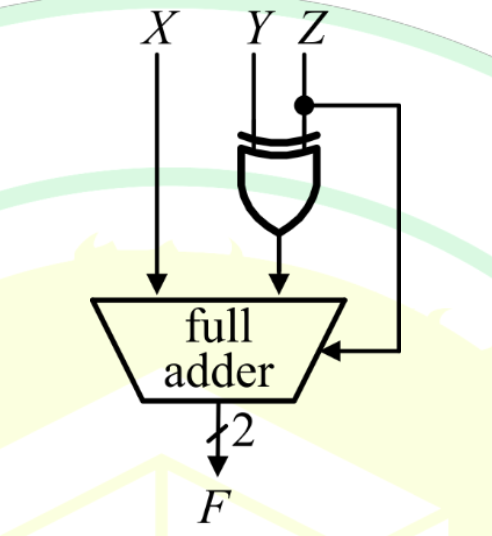
\includegraphics[width=0.4\columnwidth]{q24}
\caption{For q-24}
\label{fig:q24}
\end{figure}

\hfill{\brak{\text{GATE EC 2025}}}

\begin{enumerate}
\begin{multicols}{2}
\item an adder
\item a subtractor
\item a multiplier
\item a binary to Gray code converter
\end{multicols}
\end{enumerate}

\item Consider the function $f \colon \mathbb{R} \rightarrow \mathbb{R}$, defined as $f\brak{x} = 2x^3 - 3x^2 - 12x + 1$. Which of the following statements is/are correct? $\brak{\text{Here, } \mathbb{R} \text{ is the set of real numbers.}}$

\hfill{\brak{\text{GATE EC 2025}}}

\begin{enumerate}
\begin{multicols}{2}
\item $f$ has no global maximizer
\item $f$ has no global minimizer
\item $x = -1$ is a local minimizer of $f$
\item $x = 2$ is a local maximizer of $f$    
\end{multicols}
\end{enumerate}

\item Consider the unity-negative-feedback system shown in Figure (i) below, where gain $K \ge 0$. The root locus of this system is shown in Figure (ii) below. For what value\brak{s} of $K$ will the system in Figure (i) have a pole at $-1 + j1$?
\begin{figure}[H]
\centering
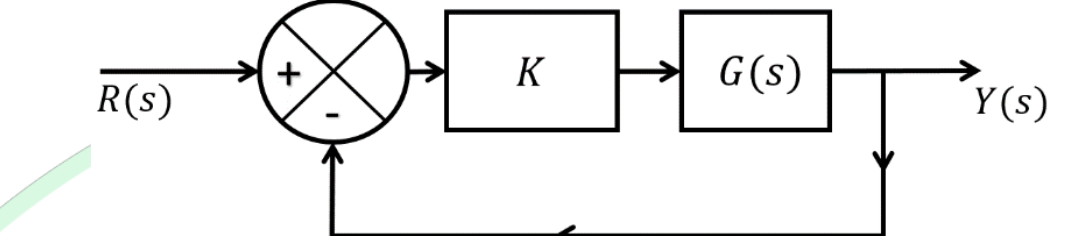
\includegraphics[width=0.4\columnwidth]{q26_i}
\end{figure}
\begin{figure}[H]
    \centering
    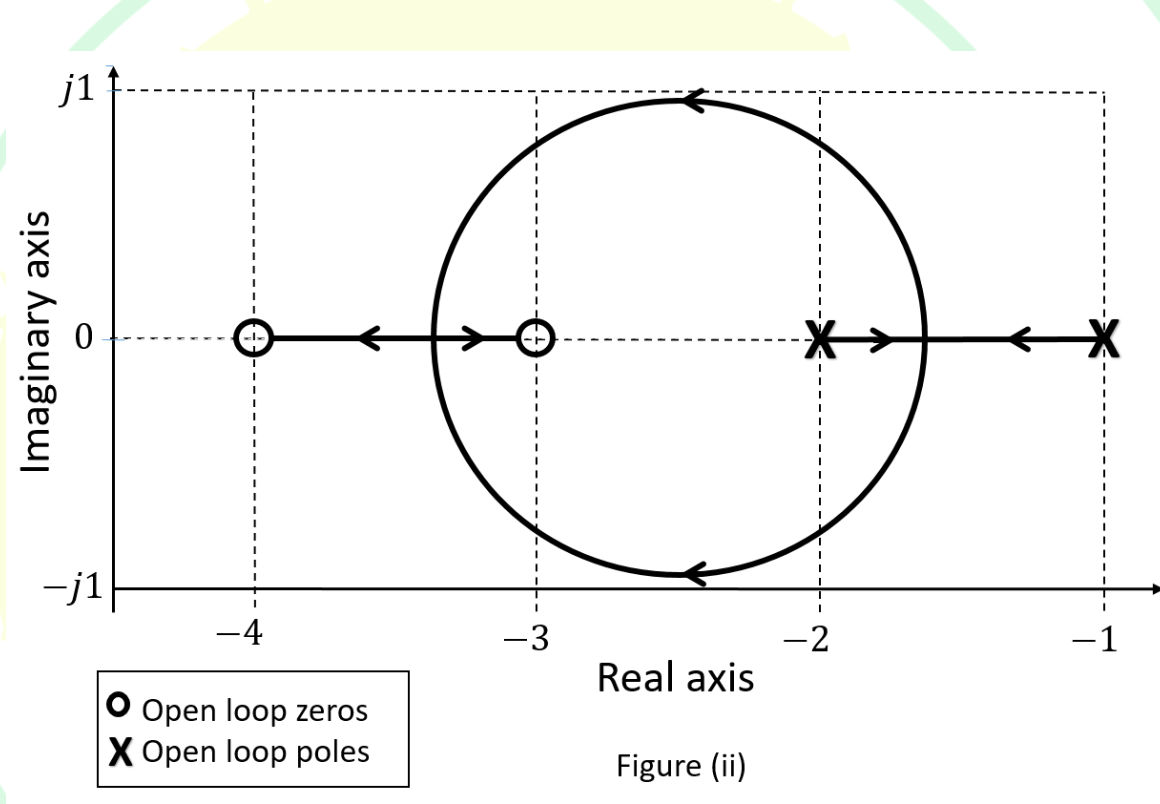
\includegraphics[width=0.6\columnwidth]{q26_ii}
    \caption*{}
    \label{fig:placeholder}
\end{figure}


\hfill{\brak{\text{GATE EC 2025}}}
\begin{multicols}{2}
\begin{enumerate}
\item $K = 5$
\item $K = 1/5$
\item For no positive value of $K$
\item For all positive values of $K$
\end{enumerate}
\end{multicols}


\item Let $x\sbrak{n}$ be a discrete-time signal whose $z$-transform is $X\brak{z}$. Which of the following statements is/are TRUE?

\hfill{\brak{\text{GATE EC 2025}}}

\begin{enumerate}
\item The discrete-time Fourier transform $\brak{DTFT}$ of $x\sbrak{n}$ always exists
\item The region of convergence $\brak{RoC}$ of $X\brak{z}$ contains neither poles nor zeros
\item The discrete-time Fourier transform $\brak{DTFT}$ exists if the region of convergence $\brak{RoC}$ contains the unit circle
\item If $x\sbrak{n} = \alpha\delta\sbrak{n}$, where $\delta\sbrak{n}$ is the unit impulse and $\alpha$ is a scalar, then the region of convergence $\brak{RoC}$ is the entire $z$-plane
\end{enumerate}

\item Consider a message signal $m\brak{t}$ which is bandlimited to $\sbrak{-W, W}$, where $W$ is in Hz. Consider the following two modulation schemes for the message signal:
\begin{itemize}
    \item Double sideband-suppressed carrier $\brak{DSB-SC}$: $f_{DSB}\brak{t} = A_c m\brak{t} \cos(2\pi f_c t)$
    \item Amplitude modulation $\brak{AM}$: $f_{AM}\brak{t} = A_c \brak{1 + \mu m\brak{t}} \cos(2\pi f_c t)$
\end{itemize}
Here, $A_c$ and $f_c$ are the amplitude and frequency $\brak{\text{in Hz}}$ of the carrier, respectively. In the case of AM, $\mu$ denotes the modulation index. Consider the following statements:
\begin{enumerate}[label=(\roman*.)]
    \item An envelope detector can be used for demodulation in the DSB-SC scheme if $m\brak{t} > 0$ for all $t$.
    \item An envelope detector can be used for demodulation in the AM scheme only if $m\brak{t} > 0$ for all $t$.
\end{enumerate}
Which of the following options is/are correct?

\hfill{\brak{\text{GATE EC 2025}}}

\begin{enumerate}
\begin{multicols}{4}
\item (i) is TRUE
\item (i) is FALSE
\item (ii) is TRUE
\item (ii) is FALSE
\end{multicols}
\end{enumerate}

\item Which of the following statements is/are TRUE with respect to an ideal opamp?

\hfill{\brak{\text{GATE EC 2025}}}

\begin{enumerate}
\begin{multicols}{2}
\item It has an infinite input resistance
\item It has an infinite output resistance
\item It has an infinite open-loop differential gain
\item It has an infinite open-loop common-mode gain
\end{multicols}
\end{enumerate}

\item Which of the following statements is/are TRUE with respect to ideal MOSFET based DC-coupled single-stage amplifiers having finite load resistors?

\hfill{\brak{\text{GATE EC 2025}}}

\begin{enumerate}
\item The common-gate amplifier has an infinite input resistance
\item The common-source amplifier has an infinite input resistance
\item The input and output voltages of the common-source amplifier are in phase
\item The input and output voltages of the common-drain amplifier are in phase
\end{enumerate}

\item Which of the following can be used as an n-type dopant for silicon? Select the correct option$\brak{s}$.

\hfill{\brak{\text{GATE EC 2025}}}

\begin{enumerate}
\begin{multicols}{4}
\item Arsenic
\item Boron
\item Gallium
\item Phosphorous
\end{multicols}
\end{enumerate}

\item The function $y\brak{t}$ satisfies $t^2y''\brak{t} - 2ty'\brak{t} + 2y\brak{t} = 0$, where $y'\brak{t}$ and $y''\brak{t}$ denote the first and second derivatives of $y\brak{t}$, respectively. Given $y'\brak{0} = 1$ and $y'\brak{1} = -1$, the maximum value of $y\brak{t}$ over $\sbrak{0,1}$ is \underline{\hspace{2cm}} $\brak{\text{rounded off to two decimal places}}$.

\hfill{\brak{\text{GATE EC 2025}}}

\item The generator matrix of a $\brak{6,3}$ binary linear block code is given by
\begin{align*}
    G = \myvec{1 & 0 & 0 & 1 & 0 & 1 \\ 0 & 1 & 0 & 0 & 1 & 1 \\ 0 & 0 & 1 & 1 & 1 & 0}.
\end{align*} 
The minimum Hamming distance $d_{min}$ between codewords equals \underline{\hspace{2cm}} $\brak{\text{answer in integer}}$.

\hfill{\brak{\text{GATE EC 2025}}}

\item All the components in the bandpass filter given in $\figref{fig:q34}$ are ideal. The lower $-3$ dB frequency of the filter is $1$ MHz. The upper $-3$ dB frequency $\brak{\text{in MHz, rounded off to the nearest integer}}$ is \underline{\hspace{2cm}}.
\begin{figure}[H]
\centering
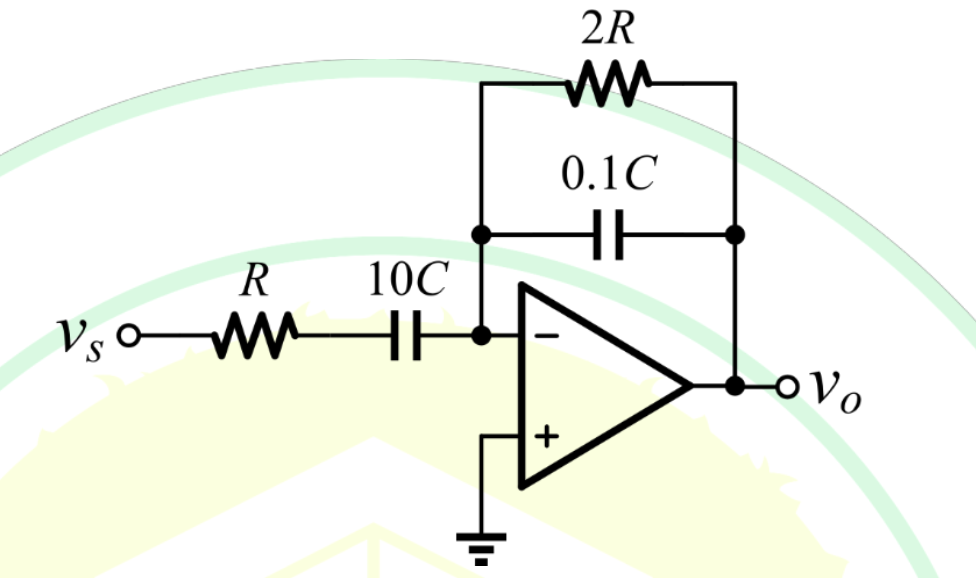
\includegraphics[width=0.5\columnwidth]{q34}
\caption{For q-34}
\label{fig:q34}
\end{figure}

\hfill{\brak{\text{GATE EC 2025}}}

\item A 4-bit weighted-resistor DAC with inputs $b_3, b_2, b_1,$ and $b_0$ \brak{MSB to LSB} is designed using an ideal opamp, as shown in $\figref{fig:q35}$. 
    The switches are closed when the corresponding input bits are logic $'1'$ and open otherwise. 
    When the input $b_3b_2b_1b_0$ changes from $1110$ to $1101$, the magnitude of the change in the output voltage $V_O$ \brak{\text{in mV, rounded off to the nearest integer}} is \underline{\hspace{2cm}}.
\begin{figure}[H]
\centering
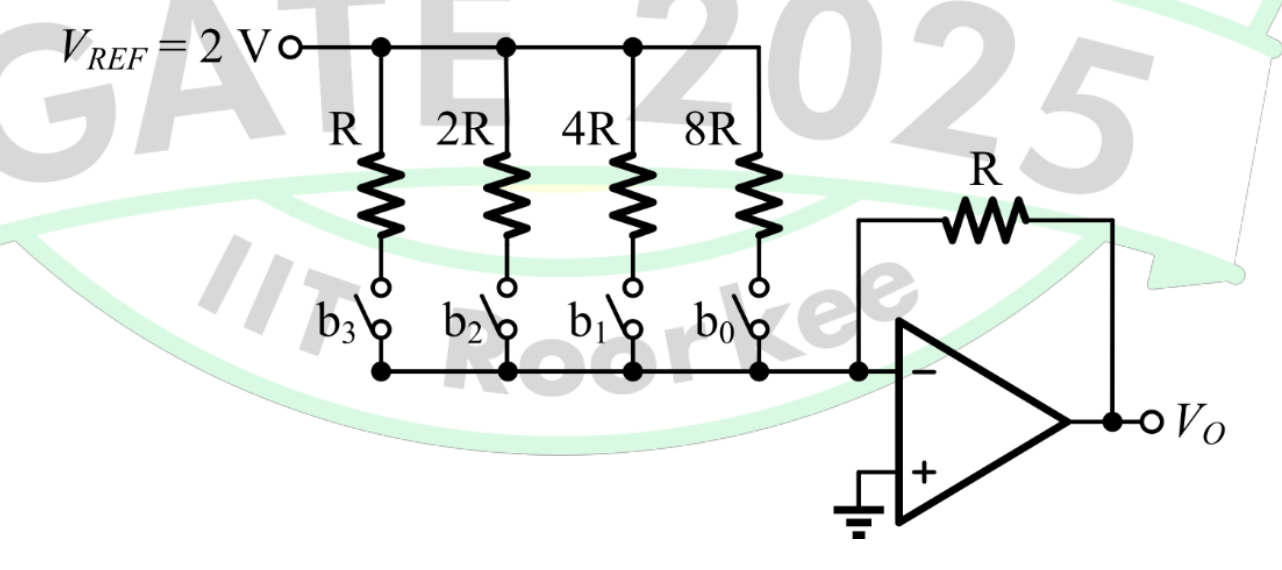
\includegraphics[width=0.7\columnwidth]{q35}
\caption{For q-35}
\label{fig:q35}
\end{figure}

\hfill{\brak{\text{GATE EC 2025}}}

\item Let $G\brak{s} = \dfrac{1}{10s^2}$ be the transfer function of a second-order system. A controller $M\brak{s}$ is connected to the system $G\brak{s}$ in the configuration shown in $\figref{fig:q36}$.
\begin{figure}[H]
\centering
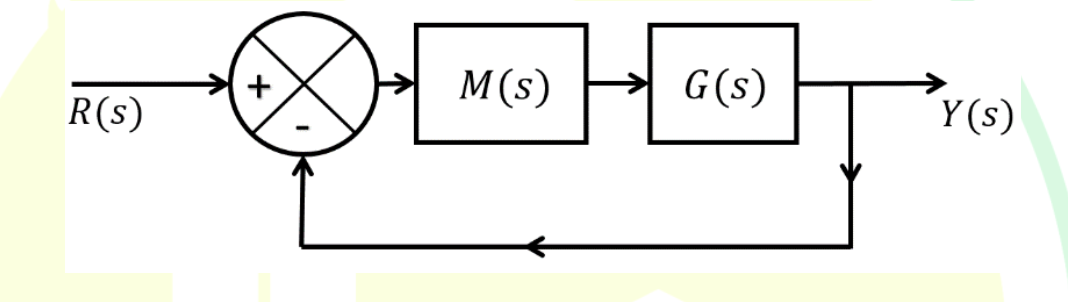
\includegraphics[width=0.5\columnwidth]{q36}
\caption{For q-36}
\label{fig:q36}
\end{figure}
Consider the following statements.
\begin{enumerate}[label=(\roman*)]
    \item There exists no controller of the form $M\brak{s} = \frac{K_I}{s}$, where $K_I$ is a positive real number, such that the closed loop system is stable.
    \item There exists at least one controller of the form $M\brak{s} = K_P + sK_D$, where $K_P$ and $K_D$ are positive real numbers, such that the closed loop system is stable.
\end{enumerate} 
Which one of the following options is correct?

\hfill{\brak{\text{GATE EC 2025}}}
\begin{multicols}{2}
\begin{enumerate}
\item (i) is TRUE and (ii) is FALSE
\item (i) is FALSE and (ii) is TRUE
\item Both (i) and (ii) are FALSE
\item Both (i) and (ii) are TRUE
\end{enumerate}    
\end{multicols}


\item Consider the polynomial $p\brak{s} = s^5 + 7s^4 + 3s^3 - 33s^2 + 2s - 40$. Let $\brak{L,I, R}$ be defined as follows.
$L$ is the number of roots of $p\brak{s}$ with negative real parts.
$I$ is the number of roots of $p\brak{s}$ that are purely imaginary.
$R$ is the number of roots of $p\brak{s}$ with positive real parts.
Which one of the following options is correct?

\hfill{\brak{\text{GATE EC 2025}}}
\begin{multicols}{2}
\begin{enumerate}
\item $L = 2, I = 2,$ and $R = 1$
\item $L = 3, I = 2,$ and $R = 0$
\item $L = 1, I = 2,$ and $R = 2$
\item $L = 0, I = 4,$ and $R = 1$
\end{enumerate}    
\end{multicols}


\item Consider a continuous-time finite-energy signal $f\brak{t}$ whose Fourier transform vanishes outside the frequency interval $\sbrak{-\omega_c, \omega_c}$, where $\omega_c$ is in rad/sec. The signal $f\brak{t}$ is uniformly sampled to obtain $y\brak{t} = f\brak{t} p\brak{t}$. Here, $p\brak{t} = \sum_{n=-\infty}^{\infty} \delta(t - \tau - nT_s)$, with $\delta\brak{t}$ being the Dirac impulse, $T_s > 0$, and $\tau > 0$. The sampled signal $y\brak{t}$ is passed through an ideal lowpass filter $h\brak{t} = \frac{\omega_c T_s \sin\brak\omega_c t}{\pi \omega_c t}$ with cutoff frequency $\omega_c$ and passband gain $T_s$. The output of the filter is given by \underline{\hspace{2cm}}.

\hfill{\brak{\text{GATE EC 2025}}}

\begin{enumerate}
\item $f\brak{t}$ if $T_s < \pi/\omega_c$
\item $f\brak{t - \tau}$ if $T_s < \pi/\omega_c$
\item $f\brak{t - \tau}$ if $T_s < 2\pi/\omega_c$
\item $T_s f\brak{t}$ if $T_s < 2\pi/\omega_c$
\end{enumerate}

\item In the circuit in $\figref{fig:q39}$, $M_1$ is an ideal AC voltmeter and $M_2$ is an ideal AC ammeter. The source voltage $\brak{\text{in Volts}}$ is $v_s\brak{t} = 100 \cos\brak{200t}$. What should be the value of the variable capacitor $C$ such that the RMS readings on $M_1$ and $M_2$ are $25$ V and $5$ A, respectively?
\begin{figure}[H]
\centering
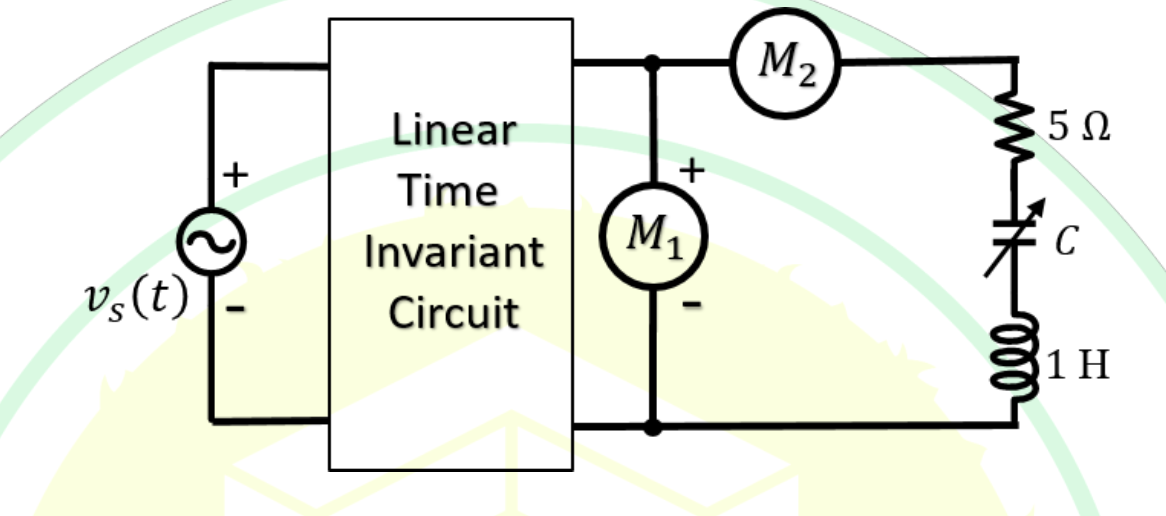
\includegraphics[width=0.5\columnwidth]{q39}
\caption{For q-39}
\label{fig:q39}
\end{figure}

\hfill{\brak{\text{GATE EC 2025}}}

\begin{enumerate}
\begin{multicols}{4}
\item 25 \textmu F
\item 4 \textmu F
\item 0.25 \textmu F
\item Insufficient information to find $C$
\end{multicols}
\end{enumerate}

\item The $Z$-parameter matrix of a two port network relates the port voltages and port currents as follows:
\begin{align*}
  \myvec{V_1 \\ V_2} = Z \myvec{I_1 \\ I_2}  
\end{align*}  
The $Z$-parameter matrix $\brak{\text{with each entry in Ohms}}$ of the network shown in $\figref{fig:q40}$ is \underline{\hspace{2cm}}.
\begin{figure}[H]
\centering
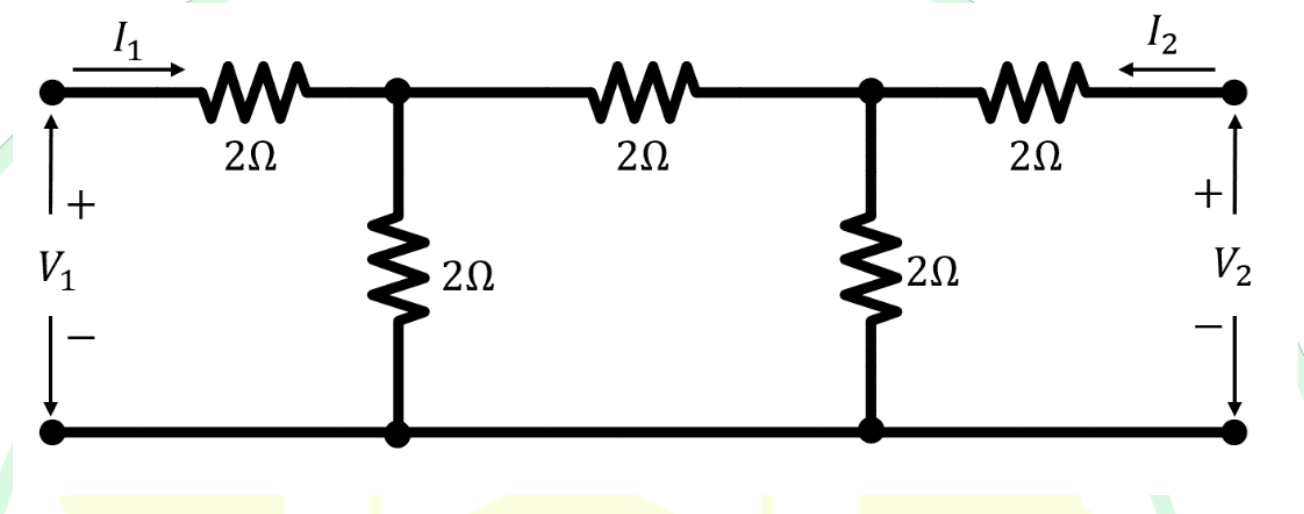
\includegraphics[width=0.6\columnwidth]{q40}
\caption{For q-40}
\label{fig:q40}
\end{figure}

\hfill{\brak{\text{GATE EC 2025}}}

\begin{enumerate}
\begin{multicols}{4}
\item $\myvec{10/3 & 2/3 \\ 2/3 & 10/3}$
\item $\myvec{2/3 & 10/3 \\ 10/3 & 2/3}$
\item $\myvec{10 & 2 \\ 2 & 10}$
\item $\myvec{10/3 & 1/3 \\ 1/3 & 10/3}$
\end{multicols}
\end{enumerate}

\item A source transmits symbol $S$ that takes values uniformly at random from the set $\cbrak{-2,0,2}$. The receiver obtains $Y = S + N$, where $N$ is a zero-mean Gaussian random variable independent of $S$. The receiver uses the maximum likelihood decoder to estimate the transmitted symbol $S$. Suppose the probability of symbol estimation error $P_e$ is expressed as follows: $P_e = \alpha P\brak{N > 1}$, where $P\brak{N > 1}$ denotes the probability that $N$ exceeds $1$. What is the value of $\alpha$?

\hfill{\brak{\text{GATE EC 2025}}}

\begin{enumerate}
\begin{multicols}{4}
\item $1/3$
\item $1$
\item $2/3$
\item $4/3$
\end{multicols}
\end{enumerate}

\item Consider a real-valued random process $f\brak{t} = \sum_{n=1}^{N} a_n p\brak{t - nT}$, where $T > 0$ and $N$ is a positive integer. Here, $p\brak{t} = 1$ for $t \in \sbrak{0, 0.5T}$ and $0$ otherwise. The coefficients $a_n$ are pairwise independent, zero-mean unit variance random variables. Read the following statements about the random process and choose the correct option.
\begin{enumerate}[label=(\roman*)]
    \item The mean of the process $f\brak{t}$ is independent of time $t$.
    \item The autocorrelation function $E[ f\brak{t}f(t + \tau)]$ is independent of time $t$ for all $\tau$.
\end{enumerate}
$\brak{\text{Here, } E[\cdot] \text{ is the expectation operation.}}$

\hfill{\brak{\text{GATE EC 2025}}}

\begin{enumerate}
\item (i) is TRUE and (ii) is FALSE
\item Both (i) and (ii) are TRUE
\item Both (i) and (ii) are FALSE
\item (i) is FALSE and (ii) is TRUE
\end{enumerate}

\item The identical MOSFETs M1 and M2 in the circuit given in $\figref{fig:q43}$ are ideal and biased in the saturation region. M1 and M2 have a transconductance $g_m$ of $5$ mS. The input signals $\brak{\text{in Volts}}$ are:
$V_1 = 2.5 + 0.01 \sin \omega t$
$V_2 = 2.5 - 0.01 \sin \omega t$
The output signal $V_3$ $\brak{\text{in Volts}}$ is \underline{\hspace{2cm}}.
\begin{figure}[H]
\centering
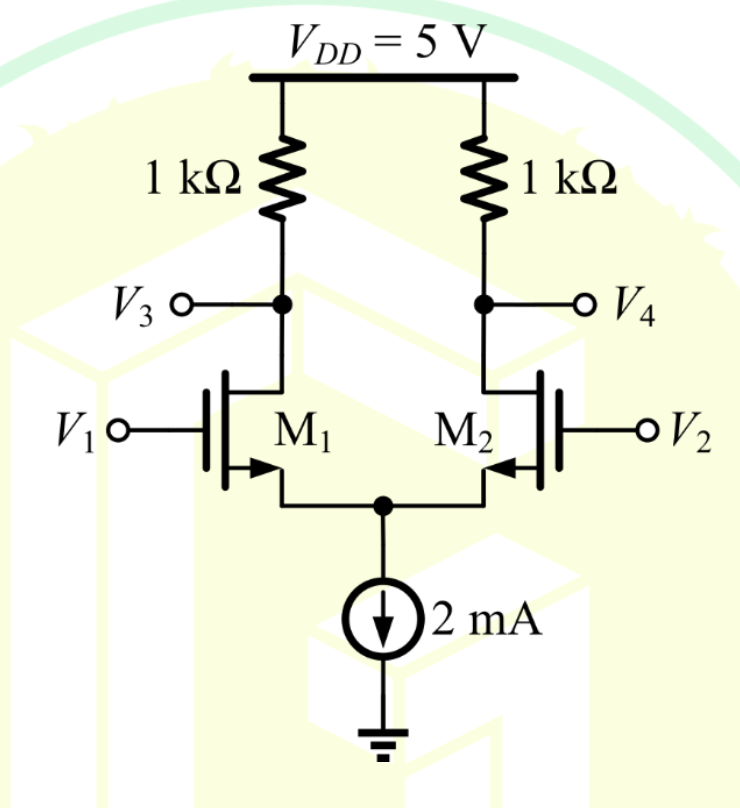
\includegraphics[width=0.5\columnwidth]{q43}
\caption{For q-43}
\label{fig:q43}
\end{figure}

\hfill{\brak{\text{GATE EC 2025}}}
\begin{multicols}{2}
\begin{enumerate}
\item $3 + 0.05 \sin \omega t$
\item $3 - 0.1 \sin \omega t$
\item $4 + 0.1 \sin \omega t$
\item $4 - 0.05 \sin \omega t$
\end{enumerate}    
\end{multicols}


\item A 10-bit analog-to-digital converter $\brak{ADC}$ has a sampling frequency of $1$ MHz and a full scale voltage of $3.3$ V. For an input sinusoidal signal with frequency $500$ kHz, the maximum SNR $\brak{\text{in dB, rounded off to two decimal places}}$ and the data rate $\brak{\text{in Mbps}}$ at the output of the ADC are \underline{\hspace{2cm}}, respectively.

\hfill{\brak{\text{GATE EC 2025}}}

\begin{enumerate}
\begin{multicols}{4}
\item $61.96$ and $10$
\item $61.96$ and $5$
\item $33.36$ and $10$
\item $33.36$ and $5$
\end{multicols}
\end{enumerate}

\item A positive-edge-triggered sequential circuit is shown in $\figref{fig:q45}$. There are no timing violations in the circuit. Input P0 is set to logic '0' and P1 is set to logic '1' at all times. The timing diagram of the inputs SEL and S are also shown below. The sequence of output Y from time T0 to T3 is \underline{\hspace{2cm}}.
\begin{figure}[H]
\centering
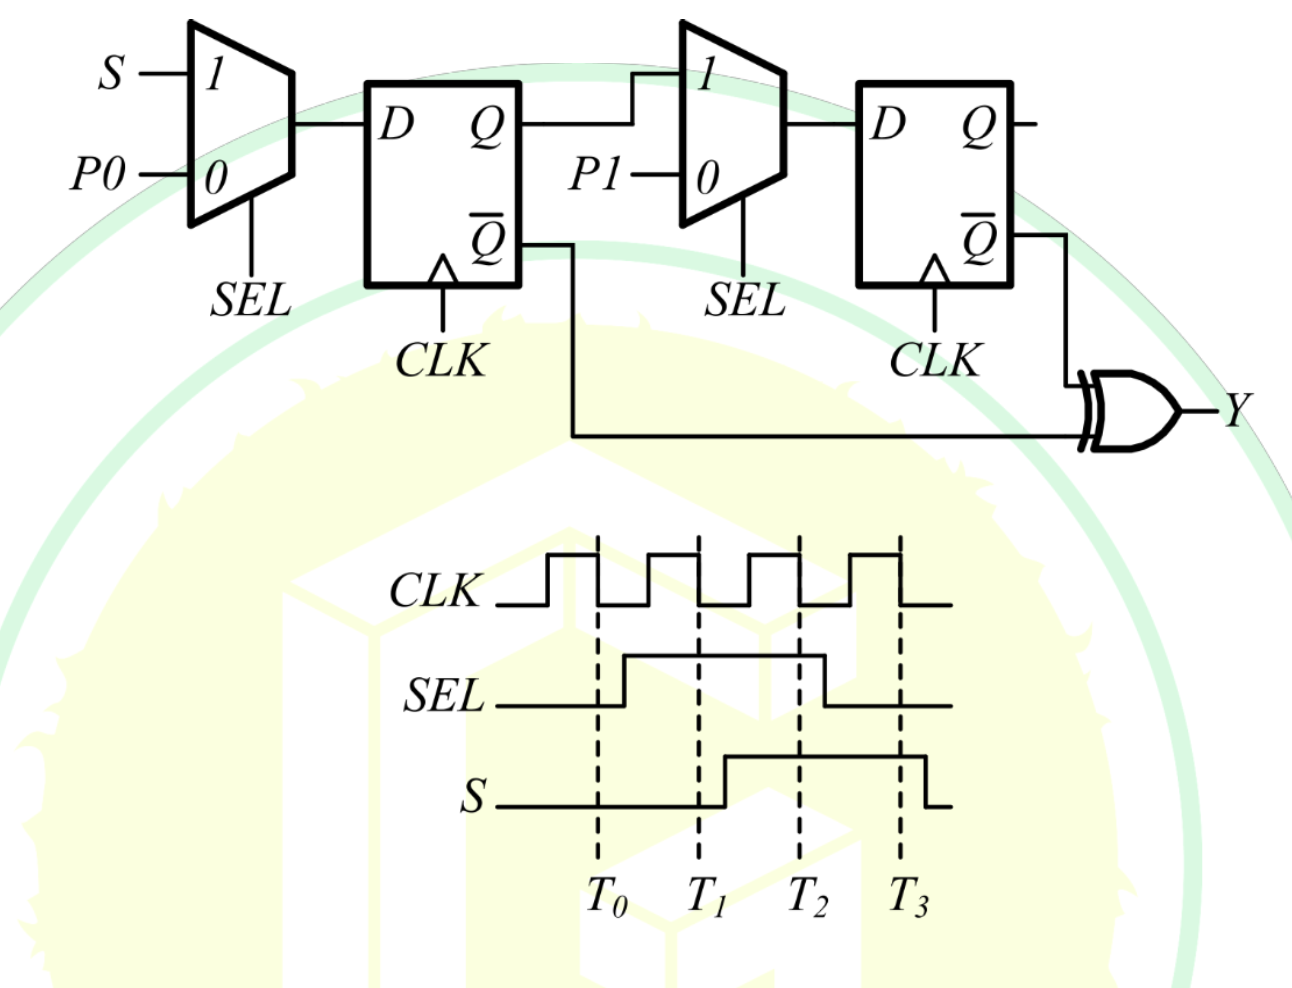
\includegraphics[width=0.5\columnwidth]{q45}
\caption{For q-45}
\label{fig:q45}
\end{figure}

\hfill{\brak{\text{GATE EC 2025}}}

\begin{enumerate}
\begin{multicols}{4}
\item $1011$
\item $0100$
\item $0010$
\item $1101$
\end{multicols}
\end{enumerate}

\item The intrinsic carrier concentration of a semiconductor is $2.5 \times 10^{16}$ /m$^3$ at $300$ K. If the electron and hole mobilities are $0.15$ m$^2$/Vs and $0.05$ m$^2$/Vs, respectively, then the intrinsic resistivity of the semiconductor $\brak{\text{in k}\ohm\text{.m}}$ at $300$ K is \underline{\hspace{2cm}}. $\brak{\text{Charge of an electron } e = 1.6 \times 10^{-19} \text{ C.}}$

\hfill{\brak{\text{GATE EC 2025}}}

\begin{enumerate}
\begin{multicols}{4}
\item $1.65$
\item $1.25$
\item $0.85$
\item $1.95$
\end{multicols}
\end{enumerate}

\item In the circuit shown in $\figref{fig:q47}$, the identical transistors Q1 and Q2 are biased in the active region with $\beta = 120$. The Zener diode is in the breakdown region with VZ = $5$ V and IZ = $25$ mA. If IL = $12$ mA and VEB1 = VEB2 = $0.7$ V, then the values of R1 and R2 $\brak{\text{in k}\ohm\text{, rounded off to one decimal place}}$ are \underline{\hspace{2cm}}, respectively.
\begin{figure}[H]
\centering
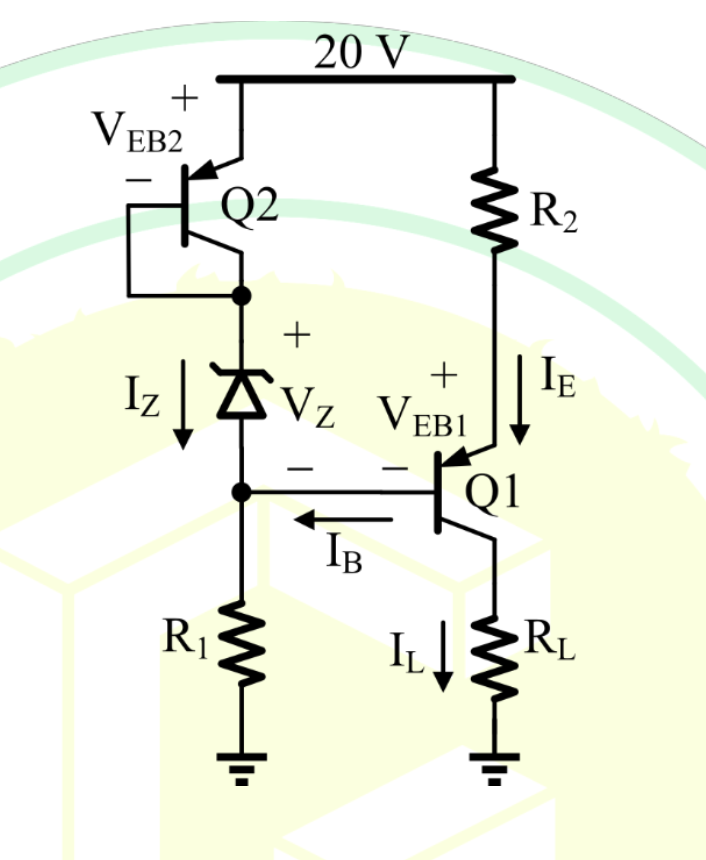
\includegraphics[width=0.3\columnwidth]{q47}
\caption{For q-47}
\label{fig:q47}
\end{figure}

\hfill{\brak{\text{GATE EC 2025}}}

\begin{enumerate}
\begin{multicols}{4}
\item $0.6$ and $0.4$
\item $1.4$ and $2.5$
\item $14.0$ and $25.0$
\item $6.0$ and $4.0$
\end{multicols}
\end{enumerate}

\item The electron mobility $\mu_n$ in a non-degenerate germanium semiconductor at $300$ K is $0.38$ m$^2$/Vs. The electron diffusivity $D_n$ at $300$ K $\brak{\text{in cm}^2\text{/s, rounded off to the nearest integer}}$ is \underline{\hspace{2cm}}. $\brak{\text{Consider the Boltzmann constant } k_B = 1.38 \times 10^{-23} \text{J/K and the charge of an electron } e = 1.6 \times 10^{-19} \text{ C.}}$

\hfill{\brak{\text{GATE EC 2025}}}

\begin{enumerate}
\begin{multicols}{4}
\item $26$
\item $98$
\item $38$
\item $10$
\end{multicols}
\end{enumerate}

\item A square metal sheet of $4$ m $\times$ $4$ m is placed on the x-y plane as shown in the $\figref{fig:q49}$ below. If the surface charge density $\brak{\text{in \textmu C/m}^2}$ on the sheet is $\rho_s(x, y) = 4\abs{y}$, then the total charge $\brak{\text{in \textmu C, rounded off to the nearest integer}}$ on the sheet is \underline{\hspace{2cm}}.
\begin{figure}[H]
\centering
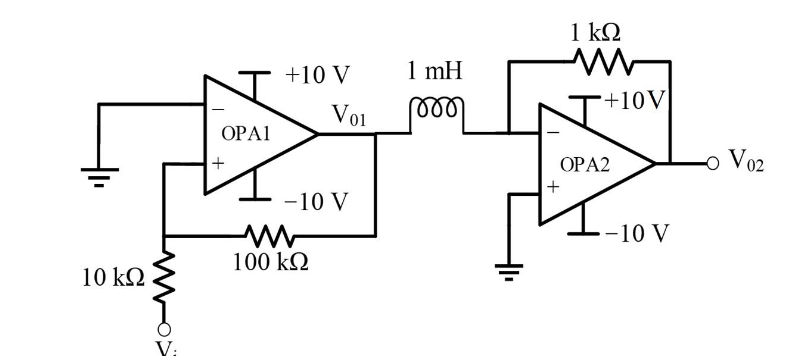
\includegraphics[width=0.4\columnwidth]{q49}
\caption{For q-49}
\label{fig:q49}
\end{figure}

\hfill{\brak{\text{GATE EC 2025}}}

\begin{enumerate}
\begin{multicols}{4}
\item $16$
\item $85$
\item $64$
\item $256$
\end{multicols}
\end{enumerate}

\item An electric field of $0.01$ V/m is applied along the length of a copper wire of circular cross-section with diameter $1$ mm. Copper has a conductivity of $5.8 \times 10^7$ S/m. The current (in Amperes, rounded off to two decimal places) flowing through the wire is \underline{\hspace{2cm}}.

\hfill{\brak{\text{GATE EC 2025}}}

\begin{enumerate}
\begin{multicols}{4}
\item $0.46$
\item $1.82$
\item $0.58$
\item $1.12$
\end{multicols}
\end{enumerate}

\item Consider a non-negative function $f\brak{x}$ which is continuous and bounded over the interval $\sbrak{2, 8}$. Let $M$ and $m$ denote, respectively, the maximum and the minimum values of $f\brak{x}$ over the interval. Among the combinations of $\alpha$ and $\beta$ given below, choose the one\brak{s} for which the inequality $\beta \le \int_2^8 f\brak{x} dx \le \alpha$ is guaranteed to hold.

\hfill{\brak{\text{GATE EC 2025}}}

\begin{enumerate}
\begin{multicols}{2}
\item $\beta = 5m, \alpha = 7M$
\item $\beta = 6m, \alpha = 5M$
\item $\beta = 7m, \alpha = 6M$
\item $\beta = 7m, \alpha = 5M$
\end{multicols}
\end{enumerate}

\item Which of the following statements involving contour integrals $\brak{\text{evaluated counter clockwise}}$ on the unit circle $C$ in the complex plane is/are TRUE?

\hfill{\brak{\text{GATE EC 2025}}}

\begin{enumerate}
\begin{multicols}{2}
\item $\oint_C e^z dz = 0$
\item $\oint_C z^n dz = 0$, where $n$ is an even integer
\item $\oint_C \cos z dz \ne 0$
\item $\oint_C \sec z dz \ne 0$
\end{multicols}
\end{enumerate}

\item Consider a system where $x_1\brak{t}, x_2\brak{t},$ and $x_3\brak{t}$ are three internal state signals and $u\brak{t}$ is the input signal. The differential equations governing the system are given by
\begin{align*}
 \frac{d}{dt} \myvec{x_1\brak{t} \\ x_2\brak{t} \\ x_3\brak{t}} = \myvec{2 & 0 & 0 \\ 0 & -2 & 0 \\ 0 & 0 & 0} \myvec{x_1\brak{t} \\ x_2\brak{t} \\ x_3\brak{t}} + \myvec{1 \\ 1 \\ 1} u\brak{t}.   
\end{align*} 
Which of the following statements is/are TRUE?

\hfill{\brak{\text{GATE EC 2025}}}

\begin{enumerate}
\item The signals $x_1\brak{t}, x_2\brak{t},$ and $x_3\brak{t}$ are bounded for all bounded inputs
\item There exists a bounded input such that at least one of the signals $x_1\brak{t}, x_2\brak{t},$ and $x_3\brak{t}$ is unbounded
\item There exists a bounded input such that the signals $x_1\brak{t}, x_2\brak{t},$ and $x_3\brak{t}$ are unbounded
\item The signals $x_1\brak{t}, x_2\brak{t},$ and $x_3\brak{t}$ are unbounded for all bounded inputs
\end{enumerate}

\item The random variable $X$ takes values in $\{-1,0,1\}$ with probabilities $P\brak{X = -1} = P\brak{X = 1} = \alpha$ and $P\brak{X = 0} = 1 - 2\alpha$, where $0 < \alpha < 1/2$. Let $g\brak{\alpha}$ denote the entropy of $X$ $\brak{\text{in bits}}$, parameterized by $\alpha$. Which of the following statements is/are TRUE?

\hfill{\brak{\text{GATE EC 2025}}}

\begin{enumerate}
\begin{multicols}{2}
\item $g\brak{0.4} > g\brak{0.3}$
\item $g\brak{0.3} > g\brak{0.4}$
\item $g\brak{0.3} > g\brak{0.25}$
\item $g\brak{0.25} > g\brak{0.3}$
\end{multicols}
\end{enumerate}

\item Let $f\brak{t}$ be a periodic signal with fundamental period $T_0 > 0$. Consider the signal $y\brak{t} = f(\alpha t)$, where $\alpha > 1$. The Fourier series expansions of $f\brak{t}$ and $y\brak{t}$ are given by
$f\brak{t} = \sum_{k=-\infty}^{\infty} c_k e^{j2\pi k t/T_0}$ and $y\brak{t} = \sum_{k=-\infty}^{\infty} d_k e^{j2\pi \alpha k t/T_0}$.
Which of the following statements is/are TRUE?

\hfill{\brak{\text{GATE EC 2025}}}

\begin{enumerate}
\item $c_k = d_k$ for all $k$
\item $y\brak{t}$ is periodic with a fundamental period $\alpha T_0$
\item $c_k = d_k/\alpha$ for all $k$
\item $y\brak{t}$ is periodic with a fundamental period $T_0/\alpha$
\end{enumerate}

\item Consider a system represented by the block diagram shown in $\figref{fig:q56}$. Which of the following signal flow graphs represent\brak{s} this system? Choose the correct option\brak{s}.
\begin{figure}[H]
\centering
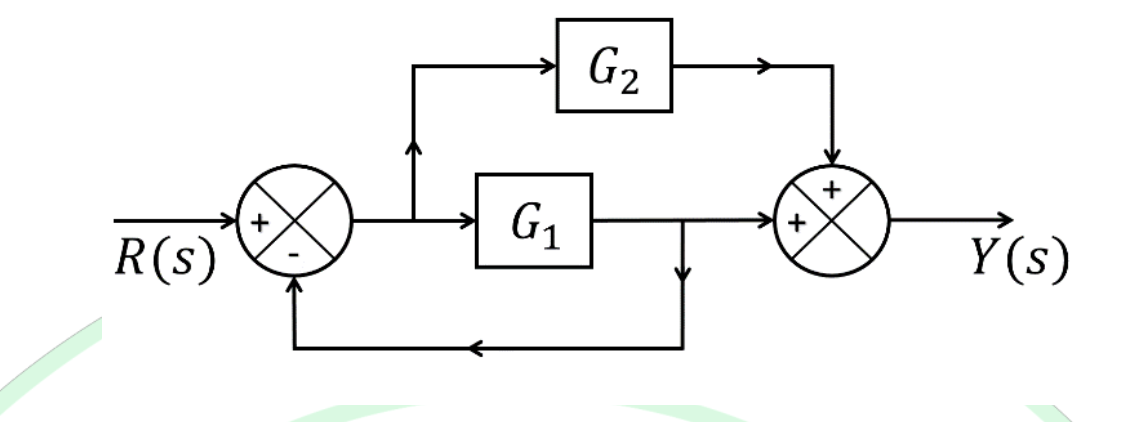
\includegraphics[width=0.5\columnwidth]{q56}
\caption{For q-56}
\label{fig:q56}
\end{figure}

\hfill{\brak{\text{GATE EC 2025}}}

\begin{multicols}{2}
\begin{enumerate}
    \item 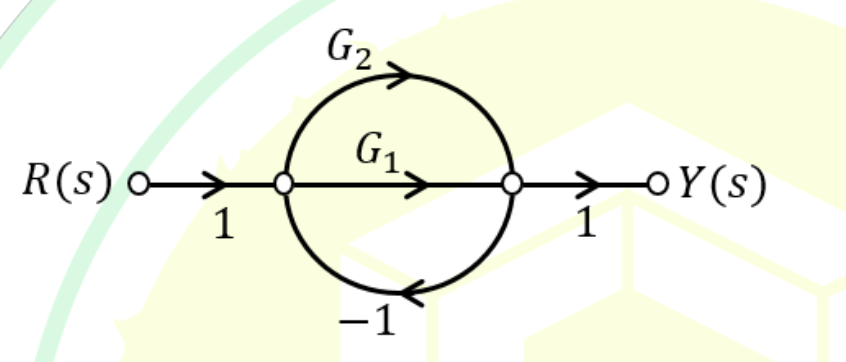
\includegraphics[width=0.6\columnwidth]{q56a.png}
    \item 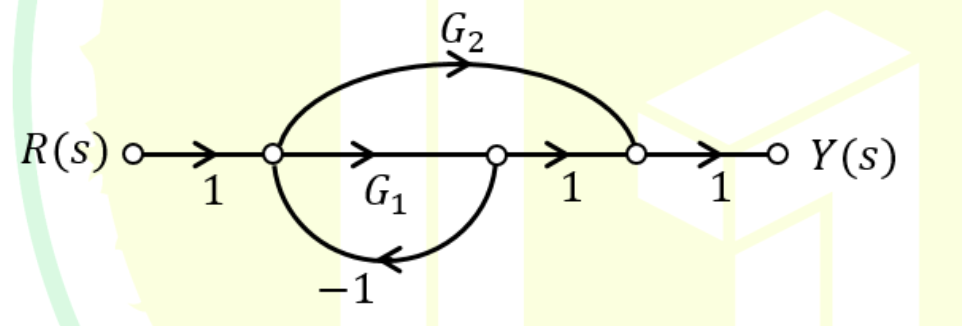
\includegraphics[width=0.6\columnwidth]{q56b.png}
    \item 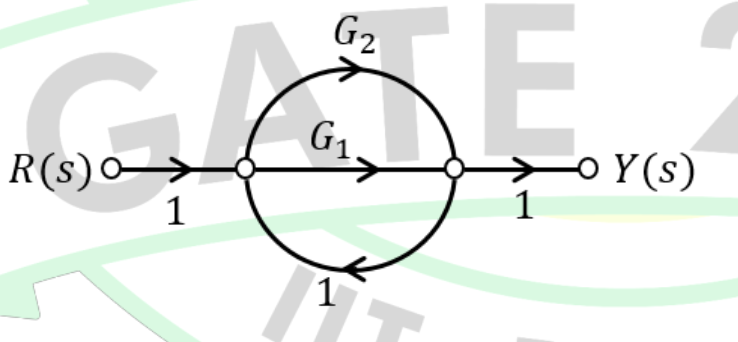
\includegraphics[width=0.6\columnwidth]{q56c.png}
    \item 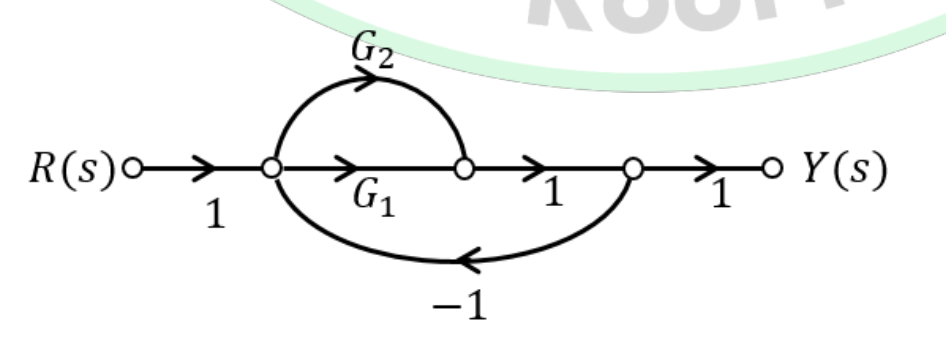
\includegraphics[width=0.6\columnwidth]{q56d.png}
\end{enumerate}
\end{multicols}

\item All the diodes in the circuit given below in $\figref{fig:q57}$ are ideal. Which of the following plots is/are correct when $V_I$ $\brak{\text{in Volts}}$ is swept from $-M$ to $M$?
\begin{figure}[H]
\centering
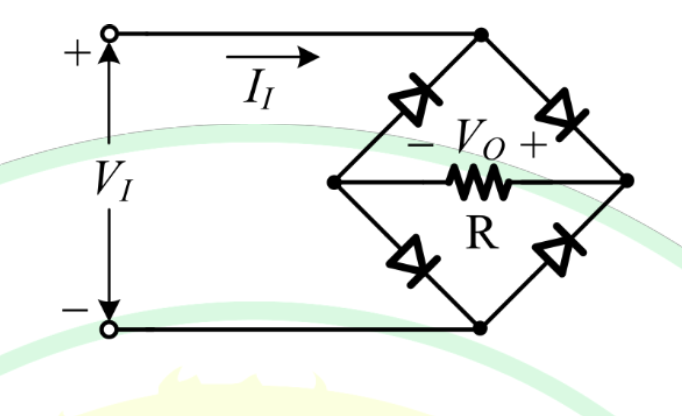
\includegraphics[width=0.4\columnwidth]{q57}
\caption{For q-57}
\label{fig:q57}
\end{figure}

\hfill{\brak{\text{GATE EC 2025}}}

\begin{multicols}{4}
\begin{enumerate}
    \item 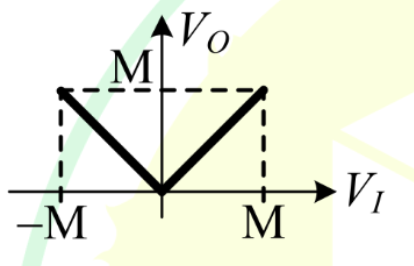
\includegraphics[width=0.3\columnwidth]{q57a.png}
    \item 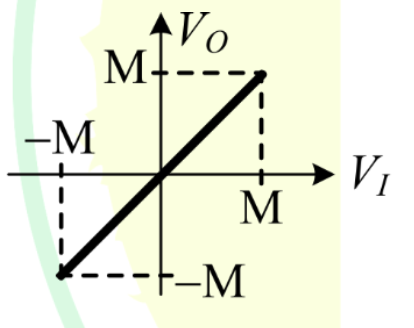
\includegraphics[width=0.3\columnwidth]{q57b.png}
    \item 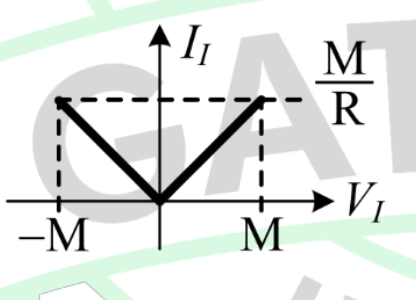
\includegraphics[width=0.3\columnwidth]{q57c.png}
    \item 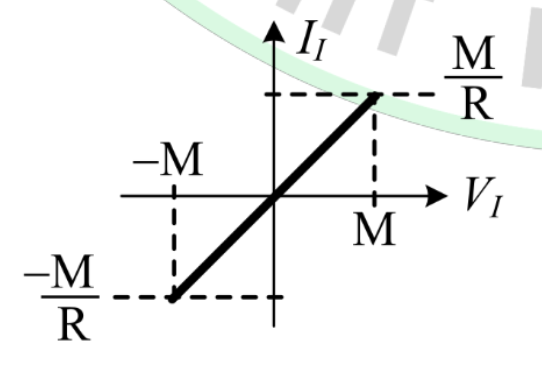
\includegraphics[width=0.3\columnwidth]{q57d.png}
\end{enumerate}
\end{multicols}

\item Two fair dice $\brak{\text{with faces labeled 1, 2, 3, 4, 5, and 6}}$ are rolled. Let the random variable $X$ denote the sum of the outcomes obtained. The expectation of $X$ is \underline{\hspace{2cm}} $\brak{\text{rounded off to two decimal places}}$.

\hfill{\brak{\text{GATE EC 2025}}}

\item Consider the vectors
$\textbf{a} = \myvec{1 \\ 1}, \textbf{b} = \myvec{0 \\ 3\sqrt{2}}$.
For real-valued scalar variable $x$, the value of
$\min_{x} \abs{\abs{\textbf{a}x - \textbf{b}}}_2$
is \underline{\hspace{2cm}} $\brak{\text{rounded off to two decimal places}}$.
$\abs{\abs{\cdot}}_2$ denotes the Euclidean norm, i.e., for $\textbf{y} = \myvec{y_1 \\ y_2}, \abs{\abs{\textbf{y}}}_2 = \sqrt{y_1^2 + y_2^2}$.

\hfill{\brak{\text{GATE EC 2025}}}

\item $X$ and $Y$ are Bernoulli random variables taking values in $\{0,1\}$. The joint probability mass function of the random variables is given by:\\
$P\brak{X = 0, Y = 0} = 0.06$\\
$P\brak{X = 0, Y = 1} = 0.14$\\
$P\brak{X = 1, Y = 0} = 0.24$\\
$P\brak{X = 1, Y = 1} = 0.56$\\
The mutual information $I(X; Y)$ is \underline{\hspace{2cm}} $\brak{\text{rounded off to two decimal places}}$.

\hfill{\brak{\text{GATE EC 2025}}}

\item The diode in the circuit shown below in $\figref{fig:q61}$ is ideal. The input voltage $\brak{\text{in Volts}}$ is given by $V_I = 10 \sin 100\pi t$, where time $t$ is in seconds. The time duration $\brak{\text{in ms, rounded off to two decimal places}}$ for which the diode is forward biased during one period of the input is \underline{\hspace{2cm}}.
\begin{figure}[H]
\centering
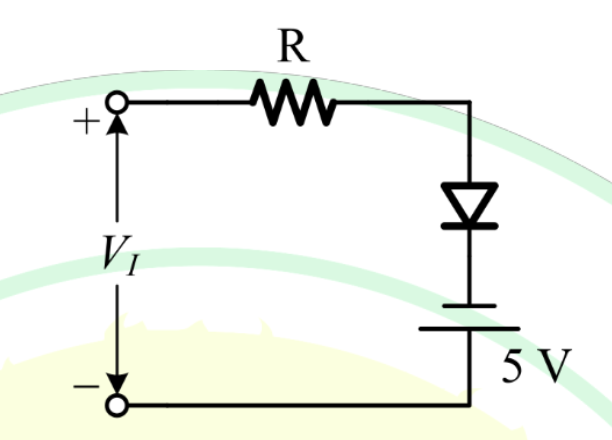
\includegraphics[width=0.4\columnwidth]{q61}
\caption{For q-61}
\label{fig:q61}
\end{figure}

\hfill{\brak{\text{GATE EC 2025}}}

\item In the circuit shown in $\figref{fig:q62}$, the AND gate has a propagation delay of $1$ ns. The edge triggered flip-flops have a set-up time of $2$ ns, a hold-time of $0$ ns, and a clock-to-Q delay of $2$ ns. The maximum clock frequency $\brak{\text{in MHz, rounded off to the nearest integer}}$ such that there are no setup violations is \underline{\hspace{2cm}}.
\begin{figure}[H]
\centering
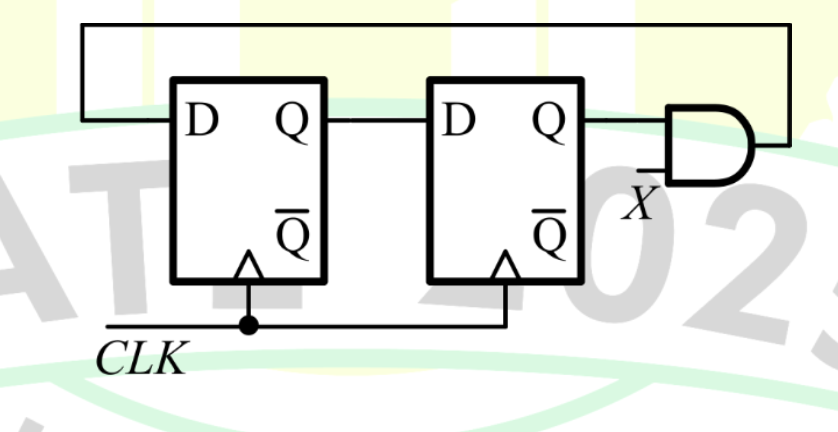
\includegraphics[width=0.5\columnwidth]{q62}
\caption{For q-62}
\label{fig:q62}
\end{figure}

\hfill{\brak{\text{GATE EC 2025}}}

\item An ideal p-n junction germanium diode has a reverse saturation current of $10$ \textmu A at $300$ K. The voltage $\brak{\text{in Volts, rounded off to two decimal places}}$ to be applied across the junction to get a forward bias current of $100$ mA at $300$ K is \underline{\hspace{2cm}}. (Consider the Boltzmann constant $k_B = 1.38 \times 10^{-23}$$ \text{J/K and the charge of an electron } e = 1.6 \times 10^{-19} \text{ C.}$)

\hfill{\brak{\text{GATE EC 2025}}}

\item A $50 \, \ohm$ lossless transmission line is terminated with a load $Z_L = (50 - j75)\,\ohm$. 
    If the average incident power on the line is $10 \,\text{mW}$, then the average power delivered to the load (in mW, rounded off to one decimal place) is \underline{\hspace{2cm}}.


\hfill{\brak{\text{GATE EC 2025}}}

\item Two resistors are connected in a circuit loop of area $5$ m$^2$, as shown in the $\figref{fig:q65}$ below. The circuit loop is placed on the x-y plane. When a time-varying magnetic flux, with flux-density $B\brak{t} = 0.5t$ $\brak{\text{in Tesla}}$, is applied along the positive z-axis, the magnitude of current I (in Amperes, rounded off to two decimal places) in the loop is $\underline{\hspace{2cm}}$.
\begin{figure}[H]
\centering
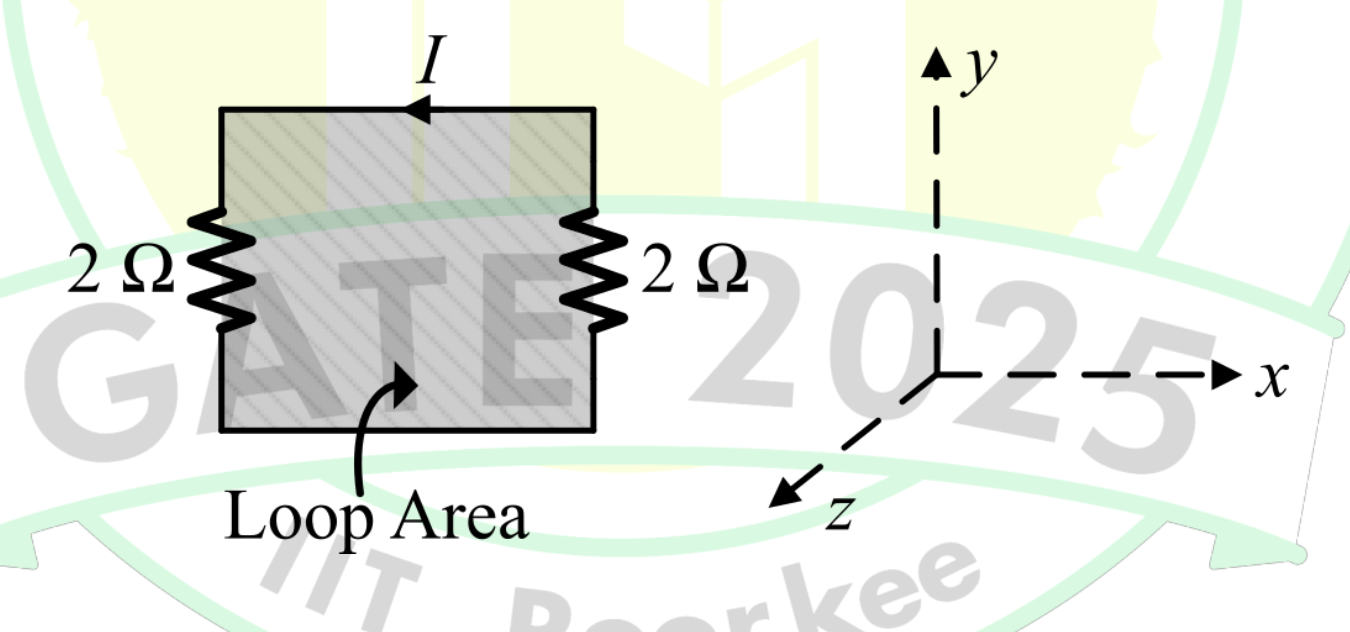
\includegraphics[width=0.5\columnwidth]{q65}
\caption{For q-65}
\label{fig:q65}
\end{figure}

\hfill{\brak{\text{GATE EC 2025}}}

\end{enumerate}

\end{document}